\documentclass[twoside]{book}

% Packages required by doxygen
\usepackage{fixltx2e}
\usepackage{calc}
\usepackage{doxygen}
\usepackage[export]{adjustbox} % also loads graphicx
\usepackage{graphicx}
\usepackage[utf8]{inputenc}
\usepackage{makeidx}
\usepackage{multicol}
\usepackage{multirow}
\PassOptionsToPackage{warn}{textcomp}
\usepackage{textcomp}
\usepackage[nointegrals]{wasysym}
\usepackage[table]{xcolor}

% Font selection
\usepackage[T1]{fontenc}
\usepackage[scaled=.90]{helvet}
\usepackage{courier}
\usepackage{amssymb}
\usepackage{sectsty}
\renewcommand{\familydefault}{\sfdefault}
\allsectionsfont{%
  \fontseries{bc}\selectfont%
  \color{darkgray}%
}
\renewcommand{\DoxyLabelFont}{%
  \fontseries{bc}\selectfont%
  \color{darkgray}%
}
\newcommand{\+}{\discretionary{\mbox{\scriptsize$\hookleftarrow$}}{}{}}

% Page & text layout
\usepackage{geometry}
\geometry{%
  a4paper,%
  top=2.5cm,%
  bottom=2.5cm,%
  left=2.5cm,%
  right=2.5cm%
}
\tolerance=750
\hfuzz=15pt
\hbadness=750
\setlength{\emergencystretch}{15pt}
\setlength{\parindent}{0cm}
\setlength{\parskip}{3ex plus 2ex minus 2ex}
\makeatletter
\renewcommand{\paragraph}{%
  \@startsection{paragraph}{4}{0ex}{-1.0ex}{1.0ex}{%
    \normalfont\normalsize\bfseries\SS@parafont%
  }%
}
\renewcommand{\subparagraph}{%
  \@startsection{subparagraph}{5}{0ex}{-1.0ex}{1.0ex}{%
    \normalfont\normalsize\bfseries\SS@subparafont%
  }%
}
\makeatother

% Headers & footers
\usepackage{fancyhdr}
\pagestyle{fancyplain}
\fancyhead[LE]{\fancyplain{}{\bfseries\thepage}}
\fancyhead[CE]{\fancyplain{}{}}
\fancyhead[RE]{\fancyplain{}{\bfseries\leftmark}}
\fancyhead[LO]{\fancyplain{}{\bfseries\rightmark}}
\fancyhead[CO]{\fancyplain{}{}}
\fancyhead[RO]{\fancyplain{}{\bfseries\thepage}}
\fancyfoot[LE]{\fancyplain{}{}}
\fancyfoot[CE]{\fancyplain{}{}}
\fancyfoot[RE]{\fancyplain{}{\bfseries\scriptsize Generated by Doxygen }}
\fancyfoot[LO]{\fancyplain{}{\bfseries\scriptsize Generated by Doxygen }}
\fancyfoot[CO]{\fancyplain{}{}}
\fancyfoot[RO]{\fancyplain{}{}}
\renewcommand{\footrulewidth}{0.4pt}
\renewcommand{\chaptermark}[1]{%
  \markboth{#1}{}%
}
\renewcommand{\sectionmark}[1]{%
  \markright{\thesection\ #1}%
}

% Indices & bibliography
\usepackage{natbib}
\usepackage[titles]{tocloft}
\setcounter{tocdepth}{3}
\setcounter{secnumdepth}{5}
\makeindex

% Hyperlinks (required, but should be loaded last)
\usepackage{ifpdf}
\ifpdf
  \usepackage[pdftex,pagebackref=true]{hyperref}
\else
  \usepackage[ps2pdf,pagebackref=true]{hyperref}
\fi
\hypersetup{%
  colorlinks=true,%
  linkcolor=blue,%
  citecolor=blue,%
  unicode%
}

% Custom commands
\newcommand{\clearemptydoublepage}{%
  \newpage{\pagestyle{empty}\cleardoublepage}%
}

\usepackage{caption}
\captionsetup{labelsep=space,justification=centering,font={bf},singlelinecheck=off,skip=4pt,position=top}

%===== C O N T E N T S =====

\begin{document}

% Titlepage & ToC
\hypersetup{pageanchor=false,
             bookmarksnumbered=true,
             pdfencoding=unicode
            }
\pagenumbering{alph}
\begin{titlepage}
\vspace*{7cm}
\begin{center}%
{\Large unagi\+\_\+server }\\
\vspace*{1cm}
{\large Generated by Doxygen 1.8.13}\\
\end{center}
\end{titlepage}
\clearemptydoublepage
\pagenumbering{roman}
\tableofcontents
\clearemptydoublepage
\pagenumbering{arabic}
\hypersetup{pageanchor=true}

%--- Begin generated contents ---
\chapter{Class Index}
\section{Class List}
Here are the classes, structs, unions and interfaces with brief descriptions\+:\begin{DoxyCompactList}
\item\contentsline{section}{\hyperlink{structcmdline__options__t}{cmdline\+\_\+options\+\_\+t} \\*サーバのコマンドラインオプションを表すデータ構造 }{\pageref{structcmdline__options__t}}{}
\item\contentsline{section}{\hyperlink{structdocument__array__t}{document\+\_\+array\+\_\+t} \\*ドキュメントの可変長配列 }{\pageref{structdocument__array__t}}{}
\item\contentsline{section}{\hyperlink{structdocument__repo__t}{document\+\_\+repo\+\_\+t} \\*ドキュメントのレポジトリ }{\pageref{structdocument__repo__t}}{}
\item\contentsline{section}{\hyperlink{structdocument__t}{document\+\_\+t} \\*1つのドキュメントを表す構造体(putされる単位) }{\pageref{structdocument__t}}{}
\item\contentsline{section}{\hyperlink{structdump__result__t}{dump\+\_\+result\+\_\+t} \\*全ドキュメントのダンプを表すデータ構造 }{\pageref{structdump__result__t}}{}
\item\contentsline{section}{\hyperlink{structoccurrence__t}{occurrence\+\_\+t} \\*文書中の検索文字列の出現(occurrence)を表すデータ }{\pageref{structoccurrence__t}}{}
\item\contentsline{section}{\hyperlink{structquery__result__t}{query\+\_\+result\+\_\+t} \\*検索結果(出現位置の集合, ストリーム)を表すデータ構造 }{\pageref{structquery__result__t}}{}
\item\contentsline{section}{\hyperlink{structrequest__t}{request\+\_\+t} \\*クライアントからのリクエストを表すデータ構造 }{\pageref{structrequest__t}}{}
\item\contentsline{section}{\hyperlink{structserver__t}{server\+\_\+t} \\*サーバを表すデータ構造 }{\pageref{structserver__t}}{}
\end{DoxyCompactList}

\chapter{File Index}
\section{File List}
Here is a list of all documented files with brief descriptions\+:\begin{DoxyCompactList}
\item\contentsline{section}{/home/tau/public\+\_\+html/lecture/operating\+\_\+systems/gen/unagi/tau/unagi/src/server/\hyperlink{document__repository_8c}{document\+\_\+repository.\+c} \\*ドキュメントを登録, 検索するレポジトリ }{\pageref{document__repository_8c}}{}
\item\contentsline{section}{/home/tau/public\+\_\+html/lecture/operating\+\_\+systems/gen/unagi/tau/unagi/src/server/\hyperlink{document__repository_8h}{document\+\_\+repository.\+h} \\*ドキュメントを登録, 検索するレポジトリ(ヘッダファイル) }{\pageref{document__repository_8h}}{}
\item\contentsline{section}{/home/tau/public\+\_\+html/lecture/operating\+\_\+systems/gen/unagi/tau/unagi/src/server/\hyperlink{unagi__server_8c}{unagi\+\_\+server.\+c} \\*Unagi server メインファイル }{\pageref{unagi__server_8c}}{}
\item\contentsline{section}{/home/tau/public\+\_\+html/lecture/operating\+\_\+systems/gen/unagi/tau/unagi/src/server/\hyperlink{unagi__utility_8c}{unagi\+\_\+utility.\+c} \\*共通に使うユーティリティ }{\pageref{unagi__utility_8c}}{}
\item\contentsline{section}{/home/tau/public\+\_\+html/lecture/operating\+\_\+systems/gen/unagi/tau/unagi/src/server/\hyperlink{unagi__utility_8h}{unagi\+\_\+utility.\+h} \\*共通に使うユーティリティ(ヘッダファイル) }{\pageref{unagi__utility_8h}}{}
\end{DoxyCompactList}

\chapter{Class Documentation}
\hypertarget{structcmdline__options__t}{}\section{cmdline\+\_\+options\+\_\+t Struct Reference}
\label{structcmdline__options__t}\index{cmdline\+\_\+options\+\_\+t@{cmdline\+\_\+options\+\_\+t}}


サーバのコマンドラインオプションを表すデータ構造  


\subsection*{Public Attributes}
\begin{DoxyCompactItemize}
\item 
int \hyperlink{structcmdline__options__t_af2128a9d51a25bcf0c62e6c380f40d5b}{port}
\item 
int \hyperlink{structcmdline__options__t_abfb9636e391795e6859dea0419dc199f}{qlen}
\item 
char $\ast$ \hyperlink{structcmdline__options__t_acaaaf78bacddf9ff0779a4956978fd06}{log}
\item 
int \hyperlink{structcmdline__options__t_a25f9087b240da0b93a4295fa5f173c88}{error}
\item 
int \hyperlink{structcmdline__options__t_ab02741e43bb19900e87caaec3a8dd794}{help}
\end{DoxyCompactItemize}


\subsection{Detailed Description}
サーバのコマンドラインオプションを表すデータ構造 

\subsection{Member Data Documentation}
\mbox{\Hypertarget{structcmdline__options__t_a25f9087b240da0b93a4295fa5f173c88}\label{structcmdline__options__t_a25f9087b240da0b93a4295fa5f173c88}} 
\index{cmdline\+\_\+options\+\_\+t@{cmdline\+\_\+options\+\_\+t}!error@{error}}
\index{error@{error}!cmdline\+\_\+options\+\_\+t@{cmdline\+\_\+options\+\_\+t}}
\subsubsection{\texorpdfstring{error}{error}}
{\footnotesize\ttfamily int cmdline\+\_\+options\+\_\+t\+::error}

コマンドライン処理でエラーが出たら1にする \mbox{\Hypertarget{structcmdline__options__t_ab02741e43bb19900e87caaec3a8dd794}\label{structcmdline__options__t_ab02741e43bb19900e87caaec3a8dd794}} 
\index{cmdline\+\_\+options\+\_\+t@{cmdline\+\_\+options\+\_\+t}!help@{help}}
\index{help@{help}!cmdline\+\_\+options\+\_\+t@{cmdline\+\_\+options\+\_\+t}}
\subsubsection{\texorpdfstring{help}{help}}
{\footnotesize\ttfamily int cmdline\+\_\+options\+\_\+t\+::help}

コマンドライン処理で\textquotesingle{}-\/h\textquotesingle{}が出たら1にする \mbox{\Hypertarget{structcmdline__options__t_acaaaf78bacddf9ff0779a4956978fd06}\label{structcmdline__options__t_acaaaf78bacddf9ff0779a4956978fd06}} 
\index{cmdline\+\_\+options\+\_\+t@{cmdline\+\_\+options\+\_\+t}!log@{log}}
\index{log@{log}!cmdline\+\_\+options\+\_\+t@{cmdline\+\_\+options\+\_\+t}}
\subsubsection{\texorpdfstring{log}{log}}
{\footnotesize\ttfamily char$\ast$ cmdline\+\_\+options\+\_\+t\+::log}

ログファイルの名前 \mbox{\Hypertarget{structcmdline__options__t_af2128a9d51a25bcf0c62e6c380f40d5b}\label{structcmdline__options__t_af2128a9d51a25bcf0c62e6c380f40d5b}} 
\index{cmdline\+\_\+options\+\_\+t@{cmdline\+\_\+options\+\_\+t}!port@{port}}
\index{port@{port}!cmdline\+\_\+options\+\_\+t@{cmdline\+\_\+options\+\_\+t}}
\subsubsection{\texorpdfstring{port}{port}}
{\footnotesize\ttfamily int cmdline\+\_\+options\+\_\+t\+::port}

接続を受け付けるポート番号(bind) \mbox{\Hypertarget{structcmdline__options__t_abfb9636e391795e6859dea0419dc199f}\label{structcmdline__options__t_abfb9636e391795e6859dea0419dc199f}} 
\index{cmdline\+\_\+options\+\_\+t@{cmdline\+\_\+options\+\_\+t}!qlen@{qlen}}
\index{qlen@{qlen}!cmdline\+\_\+options\+\_\+t@{cmdline\+\_\+options\+\_\+t}}
\subsubsection{\texorpdfstring{qlen}{qlen}}
{\footnotesize\ttfamily int cmdline\+\_\+options\+\_\+t\+::qlen}

接続要求のキュー長(listen) 

The documentation for this struct was generated from the following file\+:\begin{DoxyCompactItemize}
\item 
/home/tau/public\+\_\+html/lecture/operating\+\_\+systems/gen/unagi/tau/unagi/src/server/\hyperlink{unagi__server_8c}{unagi\+\_\+server.\+c}\end{DoxyCompactItemize}

\hypertarget{structdocument__array__t}{}\section{document\+\_\+array\+\_\+t Struct Reference}
\label{structdocument__array__t}\index{document\+\_\+array\+\_\+t@{document\+\_\+array\+\_\+t}}


ドキュメントの可変長配列  




{\ttfamily \#include $<$document\+\_\+repository.\+h$>$}



Collaboration diagram for document\+\_\+array\+\_\+t\+:\nopagebreak
\begin{figure}[H]
\begin{center}
\leavevmode
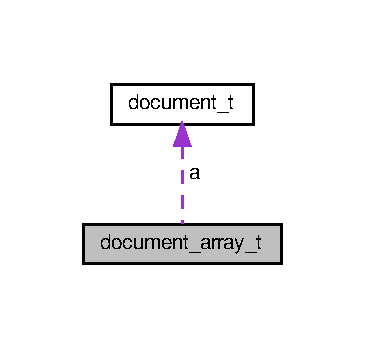
\includegraphics[width=175pt]{structdocument__array__t__coll__graph}
\end{center}
\end{figure}
\subsection*{Public Attributes}
\begin{DoxyCompactItemize}
\item 
size\+\_\+t \hyperlink{structdocument__array__t_a80cf2efb148f704dedae66740b418bab}{sz}
\item 
size\+\_\+t \hyperlink{structdocument__array__t_a5ffc023dad1cae730d69ace33c2f4853}{n}
\item 
\hyperlink{structdocument__t}{document\+\_\+t} $\ast$ \hyperlink{structdocument__array__t_a78b00a75f138da85c3342bc4cbd14ee9}{a}
\end{DoxyCompactItemize}


\subsection{Detailed Description}
ドキュメントの可変長配列 

\begin{DoxySeeAlso}{See also}
document\+\_\+array\+\_\+init 

document\+\_\+array\+\_\+destroy 

document\+\_\+array\+\_\+pushback
\end{DoxySeeAlso}
使用例

\hyperlink{structdocument__array__t}{document\+\_\+array\+\_\+t} da\mbox{[}1\mbox{]};

document\+\_\+array\+\_\+init(da);

\hyperlink{structdocument__t}{document\+\_\+t} doc = \{ ... \};

document\+\_\+array\+\_\+pushback(da, doc); 

\subsection{Member Data Documentation}
\mbox{\Hypertarget{structdocument__array__t_a78b00a75f138da85c3342bc4cbd14ee9}\label{structdocument__array__t_a78b00a75f138da85c3342bc4cbd14ee9}} 
\index{document\+\_\+array\+\_\+t@{document\+\_\+array\+\_\+t}!a@{a}}
\index{a@{a}!document\+\_\+array\+\_\+t@{document\+\_\+array\+\_\+t}}
\subsubsection{\texorpdfstring{a}{a}}
{\footnotesize\ttfamily \hyperlink{structdocument__t}{document\+\_\+t}$\ast$ document\+\_\+array\+\_\+t\+::a}

ドキュメントの配列 \mbox{\Hypertarget{structdocument__array__t_a5ffc023dad1cae730d69ace33c2f4853}\label{structdocument__array__t_a5ffc023dad1cae730d69ace33c2f4853}} 
\index{document\+\_\+array\+\_\+t@{document\+\_\+array\+\_\+t}!n@{n}}
\index{n@{n}!document\+\_\+array\+\_\+t@{document\+\_\+array\+\_\+t}}
\subsubsection{\texorpdfstring{n}{n}}
{\footnotesize\ttfamily size\+\_\+t document\+\_\+array\+\_\+t\+::n}

現在埋まっている要素数(n $<$= sz) \mbox{\Hypertarget{structdocument__array__t_a80cf2efb148f704dedae66740b418bab}\label{structdocument__array__t_a80cf2efb148f704dedae66740b418bab}} 
\index{document\+\_\+array\+\_\+t@{document\+\_\+array\+\_\+t}!sz@{sz}}
\index{sz@{sz}!document\+\_\+array\+\_\+t@{document\+\_\+array\+\_\+t}}
\subsubsection{\texorpdfstring{sz}{sz}}
{\footnotesize\ttfamily size\+\_\+t document\+\_\+array\+\_\+t\+::sz}

配列aのサイズ 

The documentation for this struct was generated from the following file\+:\begin{DoxyCompactItemize}
\item 
/home/tau/public\+\_\+html/lecture/operating\+\_\+systems/gen/unagi/tau/unagi/src/server/\hyperlink{document__repository_8h}{document\+\_\+repository.\+h}\end{DoxyCompactItemize}

\hypertarget{structdocument__repo__t}{}\section{document\+\_\+repo\+\_\+t Struct Reference}
\label{structdocument__repo__t}\index{document\+\_\+repo\+\_\+t@{document\+\_\+repo\+\_\+t}}


ドキュメントのレポジトリ  




{\ttfamily \#include $<$document\+\_\+repository.\+h$>$}



Collaboration diagram for document\+\_\+repo\+\_\+t\+:\nopagebreak
\begin{figure}[H]
\begin{center}
\leavevmode
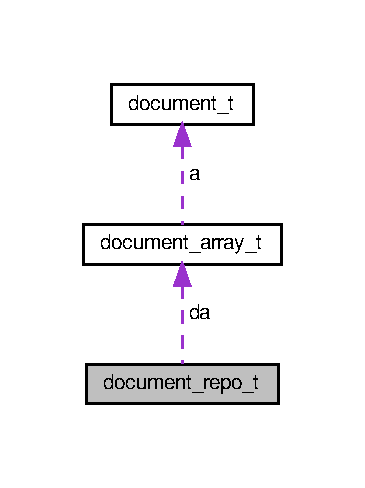
\includegraphics[width=175pt]{structdocument__repo__t__coll__graph}
\end{center}
\end{figure}
\subsection*{Public Attributes}
\begin{DoxyCompactItemize}
\item 
\hyperlink{structdocument__array__t}{document\+\_\+array\+\_\+t} \hyperlink{structdocument__repo__t_a9db2e8a3603bcf80f9500de054d5d995}{da} \mbox{[}1\mbox{]}
\end{DoxyCompactItemize}


\subsection{Detailed Description}
ドキュメントのレポジトリ 

\begin{DoxySeeAlso}{See also}
\hyperlink{document__repository_8h_ad73236d39e69cbae2e618682cb2faa4e}{document\+\_\+repo\+\_\+init} 

\hyperlink{document__repository_8h_a3e498b4e62c3223775c173a3b299f412}{document\+\_\+repo\+\_\+destroy} 

\hyperlink{document__repository_8h_aa6eebf0d0d4ec7f8d0a79dc7f061502b}{document\+\_\+repo\+\_\+add}
\end{DoxySeeAlso}
現状はドキュメントの配列そのものだが, 検索インデクスの追加など今後変更される 

\subsection{Member Data Documentation}
\mbox{\Hypertarget{structdocument__repo__t_a9db2e8a3603bcf80f9500de054d5d995}\label{structdocument__repo__t_a9db2e8a3603bcf80f9500de054d5d995}} 
\index{document\+\_\+repo\+\_\+t@{document\+\_\+repo\+\_\+t}!da@{da}}
\index{da@{da}!document\+\_\+repo\+\_\+t@{document\+\_\+repo\+\_\+t}}
\subsubsection{\texorpdfstring{da}{da}}
{\footnotesize\ttfamily \hyperlink{structdocument__array__t}{document\+\_\+array\+\_\+t} document\+\_\+repo\+\_\+t\+::da\mbox{[}1\mbox{]}}

putされたドキュメントの配列 

The documentation for this struct was generated from the following file\+:\begin{DoxyCompactItemize}
\item 
/home/tau/public\+\_\+html/lecture/operating\+\_\+systems/gen/unagi/tau/unagi/src/server/\hyperlink{document__repository_8h}{document\+\_\+repository.\+h}\end{DoxyCompactItemize}

\hypertarget{structdocument__t}{}\section{document\+\_\+t Struct Reference}
\label{structdocument__t}\index{document\+\_\+t@{document\+\_\+t}}


1つのドキュメントを表す構造体(putされる単位)  




{\ttfamily \#include $<$document\+\_\+repository.\+h$>$}

\subsection*{Public Attributes}
\begin{DoxyCompactItemize}
\item 
char $\ast$ \hyperlink{structdocument__t_adc78927f2a7a1579e3fd1c965abba435}{label}
\item 
size\+\_\+t \hyperlink{structdocument__t_aa941cb26dde0de815f368e4503a689a3}{label\+\_\+len}
\item 
char $\ast$ \hyperlink{structdocument__t_a35382946989679b4166825f1b4e2d92b}{data}
\item 
size\+\_\+t \hyperlink{structdocument__t_a39aff76b482302a6872c04a1d0fba28f}{data\+\_\+len}
\end{DoxyCompactItemize}


\subsection{Detailed Description}
1つのドキュメントを表す構造体(putされる単位) 

\begin{DoxySeeAlso}{See also}
\hyperlink{structdocument__array__t}{document\+\_\+array\+\_\+t}
\end{DoxySeeAlso}
ドキュメントは任意のラベル(典型的にはタイトル, ファイル名など)文字列と, そのドキュメントの中身で表される. 使用例\+:

char $\ast$ label = \char`\"{}野球\char`\"{}; char $\ast$ data = \char`\"{}野球はアメリカの国民的スポーツ\char`\"{}, \hyperlink{structdocument__t}{document\+\_\+t} doc = \{ label, strlen(label), data, strlen(data) \}; 

\subsection{Member Data Documentation}
\mbox{\Hypertarget{structdocument__t_a35382946989679b4166825f1b4e2d92b}\label{structdocument__t_a35382946989679b4166825f1b4e2d92b}} 
\index{document\+\_\+t@{document\+\_\+t}!data@{data}}
\index{data@{data}!document\+\_\+t@{document\+\_\+t}}
\subsubsection{\texorpdfstring{data}{data}}
{\footnotesize\ttfamily char$\ast$ document\+\_\+t\+::data}

データ(ドキュメントのテキスト) \mbox{\Hypertarget{structdocument__t_a39aff76b482302a6872c04a1d0fba28f}\label{structdocument__t_a39aff76b482302a6872c04a1d0fba28f}} 
\index{document\+\_\+t@{document\+\_\+t}!data\+\_\+len@{data\+\_\+len}}
\index{data\+\_\+len@{data\+\_\+len}!document\+\_\+t@{document\+\_\+t}}
\subsubsection{\texorpdfstring{data\+\_\+len}{data\_len}}
{\footnotesize\ttfamily size\+\_\+t document\+\_\+t\+::data\+\_\+len}

データの長さ(バイト数) \mbox{\Hypertarget{structdocument__t_adc78927f2a7a1579e3fd1c965abba435}\label{structdocument__t_adc78927f2a7a1579e3fd1c965abba435}} 
\index{document\+\_\+t@{document\+\_\+t}!label@{label}}
\index{label@{label}!document\+\_\+t@{document\+\_\+t}}
\subsubsection{\texorpdfstring{label}{label}}
{\footnotesize\ttfamily char$\ast$ document\+\_\+t\+::label}

ラベル \mbox{\Hypertarget{structdocument__t_aa941cb26dde0de815f368e4503a689a3}\label{structdocument__t_aa941cb26dde0de815f368e4503a689a3}} 
\index{document\+\_\+t@{document\+\_\+t}!label\+\_\+len@{label\+\_\+len}}
\index{label\+\_\+len@{label\+\_\+len}!document\+\_\+t@{document\+\_\+t}}
\subsubsection{\texorpdfstring{label\+\_\+len}{label\_len}}
{\footnotesize\ttfamily size\+\_\+t document\+\_\+t\+::label\+\_\+len}

ラベルの長さ(バイト数) 

The documentation for this struct was generated from the following file\+:\begin{DoxyCompactItemize}
\item 
/home/tau/public\+\_\+html/lecture/operating\+\_\+systems/gen/unagi/tau/unagi/src/server/\hyperlink{document__repository_8h}{document\+\_\+repository.\+h}\end{DoxyCompactItemize}

\hypertarget{structdump__result__t}{}\section{dump\+\_\+result\+\_\+t Struct Reference}
\label{structdump__result__t}\index{dump\+\_\+result\+\_\+t@{dump\+\_\+result\+\_\+t}}


全ドキュメントのダンプを表すデータ構造  




{\ttfamily \#include $<$document\+\_\+repository.\+h$>$}



Collaboration diagram for dump\+\_\+result\+\_\+t\+:\nopagebreak
\begin{figure}[H]
\begin{center}
\leavevmode
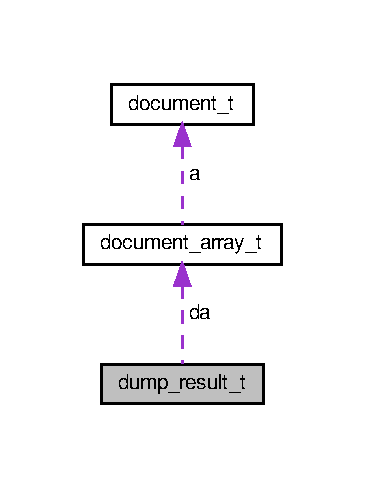
\includegraphics[width=175pt]{structdump__result__t__coll__graph}
\end{center}
\end{figure}
\subsection*{Public Attributes}
\begin{DoxyCompactItemize}
\item 
\hyperlink{structdocument__array__t}{document\+\_\+array\+\_\+t} $\ast$ \hyperlink{structdump__result__t_a8bec8965013def292a9ead629d8939a5}{da}
\item 
size\+\_\+t \hyperlink{structdump__result__t_ab5747e1016ae99e9dd3aaf13099572c7}{i}
\end{DoxyCompactItemize}


\subsection{Detailed Description}
全ドキュメントのダンプを表すデータ構造 

\begin{DoxySeeAlso}{See also}
\hyperlink{document__repository_8h_a668ef0ea9ec3a0ca0bcb98b2406eb477}{document\+\_\+repo\+\_\+dump} 

\hyperlink{document__repository_8h_a2db0fd4b412e33d8bf3549feb98b22fb}{dump\+\_\+result\+\_\+next}
\end{DoxySeeAlso}
一般に全ドキュメントは大量になりうるため, ドキュメントダンプの結果は, ドキュメントを一つずつ返すことができる データ構造とする. 具体的には, dump\+\_\+result\+\_\+next という関数で, 次のドキュメントを返すようなデータ構造とする. 従って以下のように使う.

\hyperlink{structdump__result__t}{dump\+\_\+result\+\_\+t} qr = document\+\_\+repo\+\_\+dump(repo);

while (1) \{

\hyperlink{structdocument__t}{document\+\_\+t} doc = dump\+\_\+result\+\_\+next(\&qr);

if (!doc.label) break;

... doc.\+data ...

\} 

\subsection{Member Data Documentation}
\mbox{\Hypertarget{structdump__result__t_a8bec8965013def292a9ead629d8939a5}\label{structdump__result__t_a8bec8965013def292a9ead629d8939a5}} 
\index{dump\+\_\+result\+\_\+t@{dump\+\_\+result\+\_\+t}!da@{da}}
\index{da@{da}!dump\+\_\+result\+\_\+t@{dump\+\_\+result\+\_\+t}}
\subsubsection{\texorpdfstring{da}{da}}
{\footnotesize\ttfamily \hyperlink{structdocument__array__t}{document\+\_\+array\+\_\+t}$\ast$ dump\+\_\+result\+\_\+t\+::da}

全文書の配列 \mbox{\Hypertarget{structdump__result__t_ab5747e1016ae99e9dd3aaf13099572c7}\label{structdump__result__t_ab5747e1016ae99e9dd3aaf13099572c7}} 
\index{dump\+\_\+result\+\_\+t@{dump\+\_\+result\+\_\+t}!i@{i}}
\index{i@{i}!dump\+\_\+result\+\_\+t@{dump\+\_\+result\+\_\+t}}
\subsubsection{\texorpdfstring{i}{i}}
{\footnotesize\ttfamily size\+\_\+t dump\+\_\+result\+\_\+t\+::i}

カーソル(次に返すドキュメント) 

The documentation for this struct was generated from the following file\+:\begin{DoxyCompactItemize}
\item 
/home/tau/public\+\_\+html/lecture/operating\+\_\+systems/gen/unagi/tau/unagi/src/server/\hyperlink{document__repository_8h}{document\+\_\+repository.\+h}\end{DoxyCompactItemize}

\hypertarget{structoccurrence__t}{}\section{occurrence\+\_\+t Struct Reference}
\label{structoccurrence__t}\index{occurrence\+\_\+t@{occurrence\+\_\+t}}


文書中の検索文字列の出現(occurrence)を表すデータ  




{\ttfamily \#include $<$document\+\_\+repository.\+h$>$}



Collaboration diagram for occurrence\+\_\+t\+:\nopagebreak
\begin{figure}[H]
\begin{center}
\leavevmode
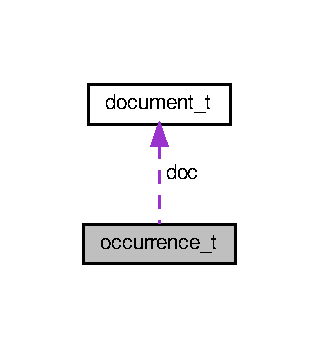
\includegraphics[width=153pt]{structoccurrence__t__coll__graph}
\end{center}
\end{figure}
\subsection*{Public Attributes}
\begin{DoxyCompactItemize}
\item 
\hyperlink{structdocument__t}{document\+\_\+t} \hyperlink{structoccurrence__t_afcff1f11f483a42c75b8a4220f395842}{doc}
\item 
size\+\_\+t \hyperlink{structoccurrence__t_a647734d7e58f6dd1c266bd4824285528}{offset}
\end{DoxyCompactItemize}


\subsection{Detailed Description}
文書中の検索文字列の出現(occurrence)を表すデータ 

ある検索文字列で検索(get)を行うと, その検索文字列が出現した 箇所が(全て)返される. \hyperlink{structoccurrence__t}{occurrence\+\_\+t} はそのうちの一つの出現を表す データ構造. どの文書に出現したかと, その中のどの位置(オフセット) に出現したかを示す. 

\subsection{Member Data Documentation}
\mbox{\Hypertarget{structoccurrence__t_afcff1f11f483a42c75b8a4220f395842}\label{structoccurrence__t_afcff1f11f483a42c75b8a4220f395842}} 
\index{occurrence\+\_\+t@{occurrence\+\_\+t}!doc@{doc}}
\index{doc@{doc}!occurrence\+\_\+t@{occurrence\+\_\+t}}
\subsubsection{\texorpdfstring{doc}{doc}}
{\footnotesize\ttfamily \hyperlink{structdocument__t}{document\+\_\+t} occurrence\+\_\+t\+::doc}

検索文字列が出現したドキュメント \mbox{\Hypertarget{structoccurrence__t_a647734d7e58f6dd1c266bd4824285528}\label{structoccurrence__t_a647734d7e58f6dd1c266bd4824285528}} 
\index{occurrence\+\_\+t@{occurrence\+\_\+t}!offset@{offset}}
\index{offset@{offset}!occurrence\+\_\+t@{occurrence\+\_\+t}}
\subsubsection{\texorpdfstring{offset}{offset}}
{\footnotesize\ttfamily size\+\_\+t occurrence\+\_\+t\+::offset}

doc中で検索文字列が出現した位置 

The documentation for this struct was generated from the following file\+:\begin{DoxyCompactItemize}
\item 
/home/tau/public\+\_\+html/lecture/operating\+\_\+systems/gen/unagi/tau/unagi/src/server/\hyperlink{document__repository_8h}{document\+\_\+repository.\+h}\end{DoxyCompactItemize}

\hypertarget{structquery__result__t}{}\section{query\+\_\+result\+\_\+t Struct Reference}
\label{structquery__result__t}\index{query\+\_\+result\+\_\+t@{query\+\_\+result\+\_\+t}}


検索結果(出現位置の集合, ストリーム)を表すデータ構造  




{\ttfamily \#include $<$document\+\_\+repository.\+h$>$}



Collaboration diagram for query\+\_\+result\+\_\+t\+:\nopagebreak
\begin{figure}[H]
\begin{center}
\leavevmode
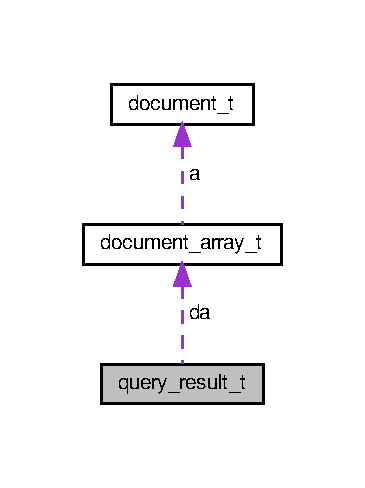
\includegraphics[width=175pt]{structquery__result__t__coll__graph}
\end{center}
\end{figure}
\subsection*{Public Attributes}
\begin{DoxyCompactItemize}
\item 
\hyperlink{structdocument__array__t}{document\+\_\+array\+\_\+t} $\ast$ \hyperlink{structquery__result__t_a4b3bddcf5a7c3a3f30ef0ae4c2fe3935}{da}
\item 
char $\ast$ \hyperlink{structquery__result__t_aa5f0530418fd600f6fb0af7ba32028bc}{query}
\item 
size\+\_\+t \hyperlink{structquery__result__t_a2b862804a4bde653fa85acdf84ae0403}{query\+\_\+len}
\item 
size\+\_\+t \hyperlink{structquery__result__t_a73621c1e37c31f8b11ee795c1ffaf808}{i}
\item 
char $\ast$ \hyperlink{structquery__result__t_ad44a1b8a87775c59260626095bb42945}{p}
\end{DoxyCompactItemize}


\subsection{Detailed Description}
検索結果(出現位置の集合, ストリーム)を表すデータ構造 

\begin{DoxySeeAlso}{See also}
\hyperlink{document__repository_8h_a8f61dbccc6befcc6affb3f6461bff262}{document\+\_\+repo\+\_\+query} 

\hyperlink{document__repository_8h_a7831dbf9173888563e4f19519d700472}{query\+\_\+result\+\_\+next}
\end{DoxySeeAlso}
一般に検索結果は, 検索文字列の出現全てであり, 大量になりうるため, 検索結果は, 出現を一つずつ返すことができる データ構造とする. 具体的には, query\+\_\+result\+\_\+next という関数で, 次の出現を返すようなデータ構造とする. 従って以下のように使う.

\hyperlink{structquery__result__t}{query\+\_\+result\+\_\+t} qr = document\+\_\+repo\+\_\+query(repo, query, query\+\_\+len);

while (1) \{

\hyperlink{structoccurrence__t}{occurrence\+\_\+t} o = query\+\_\+result\+\_\+next(\&qr);

if (!o.doc.\+label) break;

... o.\+doc.\+data\mbox{[}o.\+offset\mbox{]} から query が出現する ...

\}

この構造体の中身は以降, 検索のアルゴリズムを変える際に大きく変わる. 現状は, 全ドキュメントを順にスキャンしていくだけのアルゴリズム 

\subsection{Member Data Documentation}
\mbox{\Hypertarget{structquery__result__t_a4b3bddcf5a7c3a3f30ef0ae4c2fe3935}\label{structquery__result__t_a4b3bddcf5a7c3a3f30ef0ae4c2fe3935}} 
\index{query\+\_\+result\+\_\+t@{query\+\_\+result\+\_\+t}!da@{da}}
\index{da@{da}!query\+\_\+result\+\_\+t@{query\+\_\+result\+\_\+t}}
\subsubsection{\texorpdfstring{da}{da}}
{\footnotesize\ttfamily \hyperlink{structdocument__array__t}{document\+\_\+array\+\_\+t}$\ast$ query\+\_\+result\+\_\+t\+::da}

検索されたドキュメント配列 \mbox{\Hypertarget{structquery__result__t_a73621c1e37c31f8b11ee795c1ffaf808}\label{structquery__result__t_a73621c1e37c31f8b11ee795c1ffaf808}} 
\index{query\+\_\+result\+\_\+t@{query\+\_\+result\+\_\+t}!i@{i}}
\index{i@{i}!query\+\_\+result\+\_\+t@{query\+\_\+result\+\_\+t}}
\subsubsection{\texorpdfstring{i}{i}}
{\footnotesize\ttfamily size\+\_\+t query\+\_\+result\+\_\+t\+::i}

次に検索するドキュメントの番号(配列の添字) \mbox{\Hypertarget{structquery__result__t_ad44a1b8a87775c59260626095bb42945}\label{structquery__result__t_ad44a1b8a87775c59260626095bb42945}} 
\index{query\+\_\+result\+\_\+t@{query\+\_\+result\+\_\+t}!p@{p}}
\index{p@{p}!query\+\_\+result\+\_\+t@{query\+\_\+result\+\_\+t}}
\subsubsection{\texorpdfstring{p}{p}}
{\footnotesize\ttfamily char$\ast$ query\+\_\+result\+\_\+t\+::p}

次に検索を開始する位置 \mbox{\Hypertarget{structquery__result__t_aa5f0530418fd600f6fb0af7ba32028bc}\label{structquery__result__t_aa5f0530418fd600f6fb0af7ba32028bc}} 
\index{query\+\_\+result\+\_\+t@{query\+\_\+result\+\_\+t}!query@{query}}
\index{query@{query}!query\+\_\+result\+\_\+t@{query\+\_\+result\+\_\+t}}
\subsubsection{\texorpdfstring{query}{query}}
{\footnotesize\ttfamily char$\ast$ query\+\_\+result\+\_\+t\+::query}

検索文字列 \mbox{\Hypertarget{structquery__result__t_a2b862804a4bde653fa85acdf84ae0403}\label{structquery__result__t_a2b862804a4bde653fa85acdf84ae0403}} 
\index{query\+\_\+result\+\_\+t@{query\+\_\+result\+\_\+t}!query\+\_\+len@{query\+\_\+len}}
\index{query\+\_\+len@{query\+\_\+len}!query\+\_\+result\+\_\+t@{query\+\_\+result\+\_\+t}}
\subsubsection{\texorpdfstring{query\+\_\+len}{query\_len}}
{\footnotesize\ttfamily size\+\_\+t query\+\_\+result\+\_\+t\+::query\+\_\+len}

queryの長さ(バイト数) 

The documentation for this struct was generated from the following file\+:\begin{DoxyCompactItemize}
\item 
/home/tau/public\+\_\+html/lecture/operating\+\_\+systems/gen/unagi/tau/unagi/src/server/\hyperlink{document__repository_8h}{document\+\_\+repository.\+h}\end{DoxyCompactItemize}

\hypertarget{structrequest__t}{}\section{request\+\_\+t Struct Reference}
\label{structrequest__t}\index{request\+\_\+t@{request\+\_\+t}}


クライアントからのリクエストを表すデータ構造  


\subsection*{Public Attributes}
\begin{DoxyCompactItemize}
\item 
\hyperlink{unagi__server_8c_a30a7f6ee9120da0c95e8a1847b35a7a2}{request\+\_\+kind\+\_\+t} \hyperlink{structrequest__t_a5a7d278ddd3badff185070eea7ffdcf6}{kind}
\item 
\mbox{\Hypertarget{structrequest__t_a9b5a412828b2bbcd17f1dd0758705025}\label{structrequest__t_a9b5a412828b2bbcd17f1dd0758705025}} 
\begin{tabbing}
xx\=xx\=xx\=xx\=xx\=xx\=xx\=xx\=xx\=\kill
union \{\\
\>struct \{\\
\>\>char $\ast$ \hyperlink{structrequest__t_a29398274887826eaa815508fc159c4bb}{label}\\
\>\>size\_t \hyperlink{structrequest__t_a33f664c7c9218860358eb989281fd83d}{label\_len}\\
\>\>char $\ast$ \hyperlink{structrequest__t_aba523dc4fff06627bc840193fbafb949}{data}\\
\>\>size\_t \hyperlink{structrequest__t_a8e71192dcf1ff66483f6b4ae308f1c07}{data\_len}\\
\>\} {\bfseries put}\\
\>struct \{\\
\>\>char $\ast$ \hyperlink{structrequest__t_a1edf2a25f2884e581bd011c950ee6603}{query}\\
\>\>size\_t \hyperlink{structrequest__t_ae89af9417b7e6874716f2fe66d7112fe}{query\_len}\\
\>\} {\bfseries get}\\
\}; \\

\end{tabbing}\end{DoxyCompactItemize}


\subsection{Detailed Description}
クライアントからのリクエストを表すデータ構造 

\subsection{Member Data Documentation}
\mbox{\Hypertarget{structrequest__t_aba523dc4fff06627bc840193fbafb949}\label{structrequest__t_aba523dc4fff06627bc840193fbafb949}} 
\index{request\+\_\+t@{request\+\_\+t}!data@{data}}
\index{data@{data}!request\+\_\+t@{request\+\_\+t}}
\subsubsection{\texorpdfstring{data}{data}}
{\footnotesize\ttfamily char$\ast$ request\+\_\+t\+::data}

putされるドキュメントの中身 \mbox{\Hypertarget{structrequest__t_a8e71192dcf1ff66483f6b4ae308f1c07}\label{structrequest__t_a8e71192dcf1ff66483f6b4ae308f1c07}} 
\index{request\+\_\+t@{request\+\_\+t}!data\+\_\+len@{data\+\_\+len}}
\index{data\+\_\+len@{data\+\_\+len}!request\+\_\+t@{request\+\_\+t}}
\subsubsection{\texorpdfstring{data\+\_\+len}{data\_len}}
{\footnotesize\ttfamily size\+\_\+t request\+\_\+t\+::data\+\_\+len}

dataの長さ(バイト数) \mbox{\Hypertarget{structrequest__t_a5a7d278ddd3badff185070eea7ffdcf6}\label{structrequest__t_a5a7d278ddd3badff185070eea7ffdcf6}} 
\index{request\+\_\+t@{request\+\_\+t}!kind@{kind}}
\index{kind@{kind}!request\+\_\+t@{request\+\_\+t}}
\subsubsection{\texorpdfstring{kind}{kind}}
{\footnotesize\ttfamily \hyperlink{unagi__server_8c_a30a7f6ee9120da0c95e8a1847b35a7a2}{request\+\_\+kind\+\_\+t} request\+\_\+t\+::kind}

種類(put, get, quit, ...) \mbox{\Hypertarget{structrequest__t_a29398274887826eaa815508fc159c4bb}\label{structrequest__t_a29398274887826eaa815508fc159c4bb}} 
\index{request\+\_\+t@{request\+\_\+t}!label@{label}}
\index{label@{label}!request\+\_\+t@{request\+\_\+t}}
\subsubsection{\texorpdfstring{label}{label}}
{\footnotesize\ttfamily char$\ast$ request\+\_\+t\+::label}

putされるドキュメントのラベル(タイトル, ファイル名など任意の文字列 etc.) \mbox{\Hypertarget{structrequest__t_a33f664c7c9218860358eb989281fd83d}\label{structrequest__t_a33f664c7c9218860358eb989281fd83d}} 
\index{request\+\_\+t@{request\+\_\+t}!label\+\_\+len@{label\+\_\+len}}
\index{label\+\_\+len@{label\+\_\+len}!request\+\_\+t@{request\+\_\+t}}
\subsubsection{\texorpdfstring{label\+\_\+len}{label\_len}}
{\footnotesize\ttfamily size\+\_\+t request\+\_\+t\+::label\+\_\+len}

labelの長さ(バイト数) \mbox{\Hypertarget{structrequest__t_a1edf2a25f2884e581bd011c950ee6603}\label{structrequest__t_a1edf2a25f2884e581bd011c950ee6603}} 
\index{request\+\_\+t@{request\+\_\+t}!query@{query}}
\index{query@{query}!request\+\_\+t@{request\+\_\+t}}
\subsubsection{\texorpdfstring{query}{query}}
{\footnotesize\ttfamily char$\ast$ request\+\_\+t\+::query}

検索文字列 \mbox{\Hypertarget{structrequest__t_ae89af9417b7e6874716f2fe66d7112fe}\label{structrequest__t_ae89af9417b7e6874716f2fe66d7112fe}} 
\index{request\+\_\+t@{request\+\_\+t}!query\+\_\+len@{query\+\_\+len}}
\index{query\+\_\+len@{query\+\_\+len}!request\+\_\+t@{request\+\_\+t}}
\subsubsection{\texorpdfstring{query\+\_\+len}{query\_len}}
{\footnotesize\ttfamily size\+\_\+t request\+\_\+t\+::query\+\_\+len}

queryの長さ(バイト数) 

The documentation for this struct was generated from the following file\+:\begin{DoxyCompactItemize}
\item 
/home/tau/public\+\_\+html/lecture/operating\+\_\+systems/gen/unagi/tau/unagi/src/server/\hyperlink{unagi__server_8c}{unagi\+\_\+server.\+c}\end{DoxyCompactItemize}

\hypertarget{structserver__t}{}\section{server\+\_\+t Struct Reference}
\label{structserver__t}\index{server\+\_\+t@{server\+\_\+t}}


サーバを表すデータ構造  




Collaboration diagram for server\+\_\+t\+:\nopagebreak
\begin{figure}[H]
\begin{center}
\leavevmode
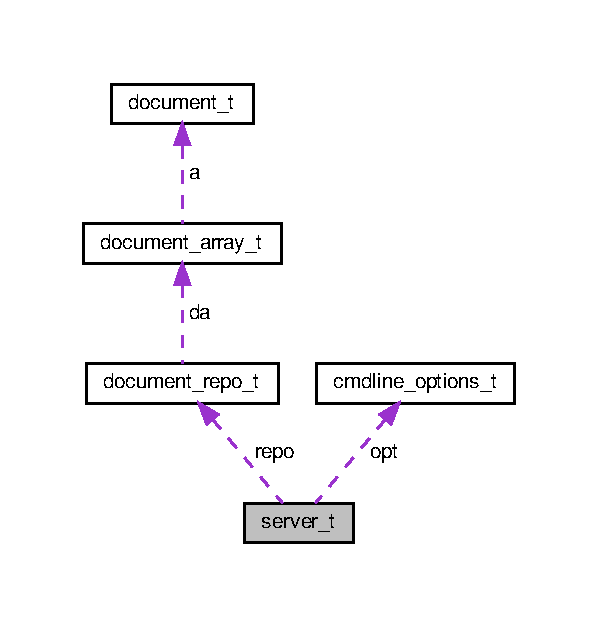
\includegraphics[width=287pt]{structserver__t__coll__graph}
\end{center}
\end{figure}
\subsection*{Public Attributes}
\begin{DoxyCompactItemize}
\item 
\hyperlink{structcmdline__options__t}{cmdline\+\_\+options\+\_\+t} \hyperlink{structserver__t_ab30d7fd534185bb41598981e1179ef61}{opt}
\item 
F\+I\+LE $\ast$ \hyperlink{structserver__t_a75cbeb1e7d454b344ac0d0b92b83d791}{log\+\_\+wp}
\item 
int \hyperlink{structserver__t_aa00bd4dd0cc9961993afa944f953b321}{server\+\_\+sock}
\item 
int \hyperlink{structserver__t_a4ad89f525db2c7f5f33e29a2413754d8}{server\+\_\+continues}
\item 
\hyperlink{structdocument__repo__t}{document\+\_\+repo\+\_\+t} \hyperlink{structserver__t_a457cf4a9e24ffd5013da271faa23e790}{repo} \mbox{[}1\mbox{]}
\end{DoxyCompactItemize}


\subsection{Detailed Description}
サーバを表すデータ構造 

\subsection{Member Data Documentation}
\mbox{\Hypertarget{structserver__t_a75cbeb1e7d454b344ac0d0b92b83d791}\label{structserver__t_a75cbeb1e7d454b344ac0d0b92b83d791}} 
\index{server\+\_\+t@{server\+\_\+t}!log\+\_\+wp@{log\+\_\+wp}}
\index{log\+\_\+wp@{log\+\_\+wp}!server\+\_\+t@{server\+\_\+t}}
\subsubsection{\texorpdfstring{log\+\_\+wp}{log\_wp}}
{\footnotesize\ttfamily F\+I\+LE$\ast$ server\+\_\+t\+::log\+\_\+wp}

ログファイルへ書き込むための\+F\+I\+L\+E$\ast$構造体 \mbox{\Hypertarget{structserver__t_ab30d7fd534185bb41598981e1179ef61}\label{structserver__t_ab30d7fd534185bb41598981e1179ef61}} 
\index{server\+\_\+t@{server\+\_\+t}!opt@{opt}}
\index{opt@{opt}!server\+\_\+t@{server\+\_\+t}}
\subsubsection{\texorpdfstring{opt}{opt}}
{\footnotesize\ttfamily \hyperlink{structcmdline__options__t}{cmdline\+\_\+options\+\_\+t} server\+\_\+t\+::opt}

コマンドラインオプション \mbox{\Hypertarget{structserver__t_a457cf4a9e24ffd5013da271faa23e790}\label{structserver__t_a457cf4a9e24ffd5013da271faa23e790}} 
\index{server\+\_\+t@{server\+\_\+t}!repo@{repo}}
\index{repo@{repo}!server\+\_\+t@{server\+\_\+t}}
\subsubsection{\texorpdfstring{repo}{repo}}
{\footnotesize\ttfamily \hyperlink{structdocument__repo__t}{document\+\_\+repo\+\_\+t} server\+\_\+t\+::repo\mbox{[}1\mbox{]}}

ドキュメントレポジトリ \mbox{\Hypertarget{structserver__t_a4ad89f525db2c7f5f33e29a2413754d8}\label{structserver__t_a4ad89f525db2c7f5f33e29a2413754d8}} 
\index{server\+\_\+t@{server\+\_\+t}!server\+\_\+continues@{server\+\_\+continues}}
\index{server\+\_\+continues@{server\+\_\+continues}!server\+\_\+t@{server\+\_\+t}}
\subsubsection{\texorpdfstring{server\+\_\+continues}{server\_continues}}
{\footnotesize\ttfamily int server\+\_\+t\+::server\+\_\+continues}

サーバが処理を続ける間1 \mbox{\Hypertarget{structserver__t_aa00bd4dd0cc9961993afa944f953b321}\label{structserver__t_aa00bd4dd0cc9961993afa944f953b321}} 
\index{server\+\_\+t@{server\+\_\+t}!server\+\_\+sock@{server\+\_\+sock}}
\index{server\+\_\+sock@{server\+\_\+sock}!server\+\_\+t@{server\+\_\+t}}
\subsubsection{\texorpdfstring{server\+\_\+sock}{server\_sock}}
{\footnotesize\ttfamily int server\+\_\+t\+::server\+\_\+sock}

接続を受け付けるソケット(socket) 

The documentation for this struct was generated from the following file\+:\begin{DoxyCompactItemize}
\item 
/home/tau/public\+\_\+html/lecture/operating\+\_\+systems/gen/unagi/tau/unagi/src/server/\hyperlink{unagi__server_8c}{unagi\+\_\+server.\+c}\end{DoxyCompactItemize}

\chapter{File Documentation}
\hypertarget{document__repository_8c}{}\section{/home/tau/public\+\_\+html/lecture/operating\+\_\+systems/gen/unagi/tau/unagi/src/server/document\+\_\+repository.c File Reference}
\label{document__repository_8c}\index{/home/tau/public\+\_\+html/lecture/operating\+\_\+systems/gen/unagi/tau/unagi/src/server/document\+\_\+repository.\+c@{/home/tau/public\+\_\+html/lecture/operating\+\_\+systems/gen/unagi/tau/unagi/src/server/document\+\_\+repository.\+c}}


ドキュメントを登録, 検索するレポジトリ  


{\ttfamily \#include $<$assert.\+h$>$}\newline
{\ttfamily \#include $<$stdlib.\+h$>$}\newline
{\ttfamily \#include $<$string.\+h$>$}\newline
{\ttfamily \#include \char`\"{}unagi\+\_\+utility.\+h\char`\"{}}\newline
{\ttfamily \#include \char`\"{}document\+\_\+repository.\+h\char`\"{}}\newline
Include dependency graph for document\+\_\+repository.\+c\+:\nopagebreak
\begin{figure}[H]
\begin{center}
\leavevmode
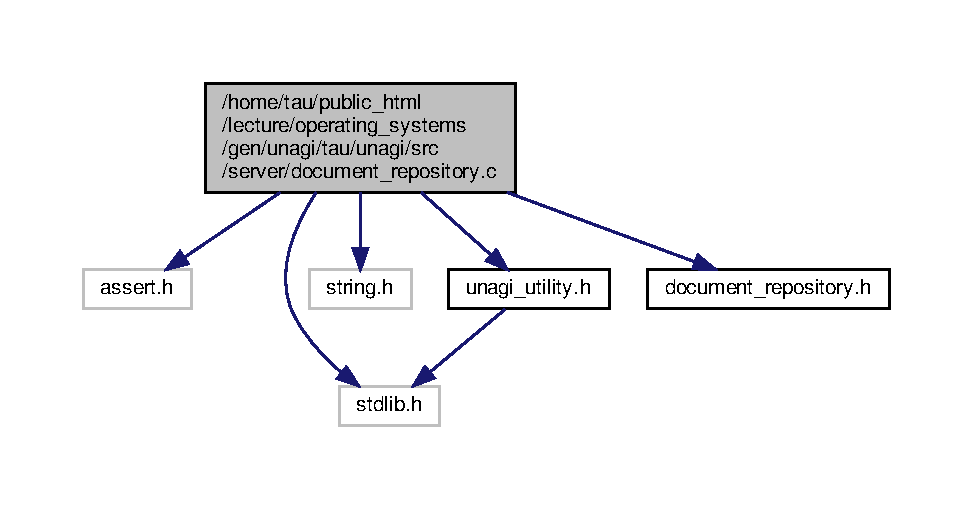
\includegraphics[width=350pt]{document__repository_8c__incl}
\end{center}
\end{figure}
\subsection*{Functions}
\begin{DoxyCompactItemize}
\item 
void \hyperlink{document__repository_8c_ad73236d39e69cbae2e618682cb2faa4e}{document\+\_\+repo\+\_\+init} (\hyperlink{structdocument__repo__t}{document\+\_\+repo\+\_\+t} $\ast$repo)
\begin{DoxyCompactList}\small\item\em ドキュメントレポジトリ(document\+\_\+repo\+\_\+t)の初期化(空にする) \end{DoxyCompactList}\item 
void \hyperlink{document__repository_8c_a3e498b4e62c3223775c173a3b299f412}{document\+\_\+repo\+\_\+destroy} (\hyperlink{structdocument__repo__t}{document\+\_\+repo\+\_\+t} $\ast$repo)
\begin{DoxyCompactList}\small\item\em ドキュメントレポジトリ(document\+\_\+repo\+\_\+t)を破壊する. メモリを開放する \end{DoxyCompactList}\item 
ssize\+\_\+t \hyperlink{document__repository_8c_aa6eebf0d0d4ec7f8d0a79dc7f061502b}{document\+\_\+repo\+\_\+add} (\hyperlink{structdocument__repo__t}{document\+\_\+repo\+\_\+t} $\ast$repo, \hyperlink{structdocument__t}{document\+\_\+t} d)
\begin{DoxyCompactList}\small\item\em ドキュメントレポジトリ(document\+\_\+repo\+\_\+t)にドキュメントを追加する \end{DoxyCompactList}\item 
\hyperlink{structquery__result__t}{query\+\_\+result\+\_\+t} \hyperlink{document__repository_8c_a8f61dbccc6befcc6affb3f6461bff262}{document\+\_\+repo\+\_\+query} (\hyperlink{structdocument__repo__t}{document\+\_\+repo\+\_\+t} $\ast$repo, char $\ast$query, size\+\_\+t query\+\_\+len)
\begin{DoxyCompactList}\small\item\em ドキュメントレポジトリから指定文字列(query)を検索. \end{DoxyCompactList}\item 
\hyperlink{structoccurrence__t}{occurrence\+\_\+t} \hyperlink{document__repository_8c_a7831dbf9173888563e4f19519d700472}{query\+\_\+result\+\_\+next} (\hyperlink{structquery__result__t}{query\+\_\+result\+\_\+t} $\ast$qr)
\begin{DoxyCompactList}\small\item\em document\+\_\+repo\+\_\+query で得られた検索結果から, 次の出現位置を得る \end{DoxyCompactList}\item 
size\+\_\+t \hyperlink{document__repository_8c_a81fe0bb9c8482bbaa25b277dbf1a22ad}{document\+\_\+repo\+\_\+queryc} (\hyperlink{structdocument__repo__t}{document\+\_\+repo\+\_\+t} $\ast$repo, char $\ast$query, size\+\_\+t query\+\_\+len)
\begin{DoxyCompactList}\small\item\em ドキュメントレポジトリから指定文字列(query)を検索しその出現回数 (のみ)を返す \end{DoxyCompactList}\item 
\hyperlink{structdump__result__t}{dump\+\_\+result\+\_\+t} \hyperlink{document__repository_8c_a668ef0ea9ec3a0ca0bcb98b2406eb477}{document\+\_\+repo\+\_\+dump} (\hyperlink{structdocument__repo__t}{document\+\_\+repo\+\_\+t} $\ast$repo)
\begin{DoxyCompactList}\small\item\em 全ドキュメントのダンプを表すデータ構造 \end{DoxyCompactList}\item 
\mbox{\Hypertarget{document__repository_8c_affebc850b20de4382fff4a039f59c5a7}\label{document__repository_8c_affebc850b20de4382fff4a039f59c5a7}} 
size\+\_\+t \hyperlink{document__repository_8c_affebc850b20de4382fff4a039f59c5a7}{document\+\_\+repo\+\_\+n\+\_\+docs} (\hyperlink{structdocument__repo__t}{document\+\_\+repo\+\_\+t} $\ast$repo)
\begin{DoxyCompactList}\small\item\em 全ドキュメント数を取得する. \end{DoxyCompactList}\item 
\mbox{\Hypertarget{document__repository_8c_a2db0fd4b412e33d8bf3549feb98b22fb}\label{document__repository_8c_a2db0fd4b412e33d8bf3549feb98b22fb}} 
\hyperlink{structdocument__t}{document\+\_\+t} \hyperlink{document__repository_8c_a2db0fd4b412e33d8bf3549feb98b22fb}{dump\+\_\+result\+\_\+next} (\hyperlink{structdump__result__t}{dump\+\_\+result\+\_\+t} $\ast$dr)
\begin{DoxyCompactList}\small\item\em document\+\_\+repo\+\_\+dump が返した \hyperlink{structdump__result__t}{dump\+\_\+result\+\_\+t} から, 次のドキュメントを返す. \end{DoxyCompactList}\end{DoxyCompactItemize}


\subsection{Detailed Description}
ドキュメントを登録, 検索するレポジトリ 

\begin{DoxyAuthor}{Author}
田浦 
\end{DoxyAuthor}
\begin{DoxyDate}{Date}
Oct. 8, 2018 
\end{DoxyDate}


\subsection{Function Documentation}
\mbox{\Hypertarget{document__repository_8c_aa6eebf0d0d4ec7f8d0a79dc7f061502b}\label{document__repository_8c_aa6eebf0d0d4ec7f8d0a79dc7f061502b}} 
\index{document\+\_\+repository.\+c@{document\+\_\+repository.\+c}!document\+\_\+repo\+\_\+add@{document\+\_\+repo\+\_\+add}}
\index{document\+\_\+repo\+\_\+add@{document\+\_\+repo\+\_\+add}!document\+\_\+repository.\+c@{document\+\_\+repository.\+c}}
\subsubsection{\texorpdfstring{document\+\_\+repo\+\_\+add()}{document\_repo\_add()}}
{\footnotesize\ttfamily ssize\+\_\+t document\+\_\+repo\+\_\+add (\begin{DoxyParamCaption}\item[{\hyperlink{structdocument__repo__t}{document\+\_\+repo\+\_\+t} $\ast$}]{repo,  }\item[{\hyperlink{structdocument__t}{document\+\_\+t}}]{d }\end{DoxyParamCaption})}



ドキュメントレポジトリ(document\+\_\+repo\+\_\+t)にドキュメントを追加する 

\begin{DoxyReturn}{Returns}
成功したら, 非負の整数. 失敗(メモリ割り当て失敗)したら-\/1.
\end{DoxyReturn}
\begin{DoxySeeAlso}{See also}
\hyperlink{document__repository_8c_ad73236d39e69cbae2e618682cb2faa4e}{document\+\_\+repo\+\_\+init} 

\hyperlink{document__repository_8c_a3e498b4e62c3223775c173a3b299f412}{document\+\_\+repo\+\_\+destroy} 

\hyperlink{structdocument__repo__t}{document\+\_\+repo\+\_\+t} 
\end{DoxySeeAlso}
\mbox{\Hypertarget{document__repository_8c_a3e498b4e62c3223775c173a3b299f412}\label{document__repository_8c_a3e498b4e62c3223775c173a3b299f412}} 
\index{document\+\_\+repository.\+c@{document\+\_\+repository.\+c}!document\+\_\+repo\+\_\+destroy@{document\+\_\+repo\+\_\+destroy}}
\index{document\+\_\+repo\+\_\+destroy@{document\+\_\+repo\+\_\+destroy}!document\+\_\+repository.\+c@{document\+\_\+repository.\+c}}
\subsubsection{\texorpdfstring{document\+\_\+repo\+\_\+destroy()}{document\_repo\_destroy()}}
{\footnotesize\ttfamily void document\+\_\+repo\+\_\+destroy (\begin{DoxyParamCaption}\item[{\hyperlink{structdocument__repo__t}{document\+\_\+repo\+\_\+t} $\ast$}]{repo }\end{DoxyParamCaption})}



ドキュメントレポジトリ(document\+\_\+repo\+\_\+t)を破壊する. メモリを開放する 

\begin{DoxySeeAlso}{See also}
\hyperlink{document__repository_8c_ad73236d39e69cbae2e618682cb2faa4e}{document\+\_\+repo\+\_\+init} 

\hyperlink{document__repository_8c_aa6eebf0d0d4ec7f8d0a79dc7f061502b}{document\+\_\+repo\+\_\+add} 

\hyperlink{structdocument__repo__t}{document\+\_\+repo\+\_\+t} 
\end{DoxySeeAlso}
\mbox{\Hypertarget{document__repository_8c_a668ef0ea9ec3a0ca0bcb98b2406eb477}\label{document__repository_8c_a668ef0ea9ec3a0ca0bcb98b2406eb477}} 
\index{document\+\_\+repository.\+c@{document\+\_\+repository.\+c}!document\+\_\+repo\+\_\+dump@{document\+\_\+repo\+\_\+dump}}
\index{document\+\_\+repo\+\_\+dump@{document\+\_\+repo\+\_\+dump}!document\+\_\+repository.\+c@{document\+\_\+repository.\+c}}
\subsubsection{\texorpdfstring{document\+\_\+repo\+\_\+dump()}{document\_repo\_dump()}}
{\footnotesize\ttfamily \hyperlink{structdump__result__t}{dump\+\_\+result\+\_\+t} document\+\_\+repo\+\_\+dump (\begin{DoxyParamCaption}\item[{\hyperlink{structdocument__repo__t}{document\+\_\+repo\+\_\+t} $\ast$}]{repo }\end{DoxyParamCaption})}



全ドキュメントのダンプを表すデータ構造 

\begin{DoxySeeAlso}{See also}
\hyperlink{document__repository_8c_a668ef0ea9ec3a0ca0bcb98b2406eb477}{document\+\_\+repo\+\_\+dump} 

\hyperlink{document__repository_8c_a2db0fd4b412e33d8bf3549feb98b22fb}{dump\+\_\+result\+\_\+next}
\end{DoxySeeAlso}
一般に全ドキュメントは大量になりうるため, ドキュメントダンプの結果は, ドキュメントを一つずつ返すことができる データ構造とする. 具体的には, dump\+\_\+result\+\_\+next という関数で, 次のドキュメントを返すようなデータ構造とする. 従って以下のように使う.

\hyperlink{structdump__result__t}{dump\+\_\+result\+\_\+t} qr = document\+\_\+repo\+\_\+dump(repo);

while (1) \{

\hyperlink{structdocument__t}{document\+\_\+t} doc = dump\+\_\+result\+\_\+next(\&qr);

if (!doc.label) break;

... doc.\+data ...

\} 全ドキュメントのダンプを取得する

\hyperlink{structdump__result__t}{dump\+\_\+result\+\_\+t} 型の構造体を返す. その構造体は, dump\+\_\+result\+\_\+next(..) 関数を次々と呼ぶことで, 次々に ドキュメントを返す. \mbox{\Hypertarget{document__repository_8c_ad73236d39e69cbae2e618682cb2faa4e}\label{document__repository_8c_ad73236d39e69cbae2e618682cb2faa4e}} 
\index{document\+\_\+repository.\+c@{document\+\_\+repository.\+c}!document\+\_\+repo\+\_\+init@{document\+\_\+repo\+\_\+init}}
\index{document\+\_\+repo\+\_\+init@{document\+\_\+repo\+\_\+init}!document\+\_\+repository.\+c@{document\+\_\+repository.\+c}}
\subsubsection{\texorpdfstring{document\+\_\+repo\+\_\+init()}{document\_repo\_init()}}
{\footnotesize\ttfamily void document\+\_\+repo\+\_\+init (\begin{DoxyParamCaption}\item[{\hyperlink{structdocument__repo__t}{document\+\_\+repo\+\_\+t} $\ast$}]{repo }\end{DoxyParamCaption})}



ドキュメントレポジトリ(document\+\_\+repo\+\_\+t)の初期化(空にする) 

\begin{DoxySeeAlso}{See also}
\hyperlink{document__repository_8c_a3e498b4e62c3223775c173a3b299f412}{document\+\_\+repo\+\_\+destroy} 

\hyperlink{document__repository_8c_aa6eebf0d0d4ec7f8d0a79dc7f061502b}{document\+\_\+repo\+\_\+add} 

\hyperlink{structdocument__repo__t}{document\+\_\+repo\+\_\+t} 
\end{DoxySeeAlso}
\mbox{\Hypertarget{document__repository_8c_a8f61dbccc6befcc6affb3f6461bff262}\label{document__repository_8c_a8f61dbccc6befcc6affb3f6461bff262}} 
\index{document\+\_\+repository.\+c@{document\+\_\+repository.\+c}!document\+\_\+repo\+\_\+query@{document\+\_\+repo\+\_\+query}}
\index{document\+\_\+repo\+\_\+query@{document\+\_\+repo\+\_\+query}!document\+\_\+repository.\+c@{document\+\_\+repository.\+c}}
\subsubsection{\texorpdfstring{document\+\_\+repo\+\_\+query()}{document\_repo\_query()}}
{\footnotesize\ttfamily \hyperlink{structquery__result__t}{query\+\_\+result\+\_\+t} document\+\_\+repo\+\_\+query (\begin{DoxyParamCaption}\item[{\hyperlink{structdocument__repo__t}{document\+\_\+repo\+\_\+t} $\ast$}]{repo,  }\item[{char $\ast$}]{query,  }\item[{size\+\_\+t}]{query\+\_\+len }\end{DoxyParamCaption})}



ドキュメントレポジトリから指定文字列(query)を検索. 

\begin{DoxyReturn}{Returns}
検索結果(query\+\_\+result\+\_\+t) 
\end{DoxyReturn}
\begin{DoxySeeAlso}{See also}
\hyperlink{structquery__result__t}{query\+\_\+result\+\_\+t} 

\hyperlink{document__repository_8c_a7831dbf9173888563e4f19519d700472}{query\+\_\+result\+\_\+next} 

\hyperlink{document__repository_8c_aa6eebf0d0d4ec7f8d0a79dc7f061502b}{document\+\_\+repo\+\_\+add}
\end{DoxySeeAlso}
ドキュメントレポジトリ内の全ドキュメント(これまでに document\+\_\+repo\+\_\+add されたすべてのドキュメント)から検索文字列 query の出現を検索する. query\+\_\+result\+\_\+next は, そこから全ての出現位置を取 得することができるようなデータである. 詳しくは, \hyperlink{structquery__result__t}{query\+\_\+result\+\_\+t} のド キュメントを参照 
\begin{DoxyParams}{Parameters}
{\em repo} & 検索対象のドキュメントレポジトリ \\
\hline
{\em query} & 検索文字列 \\
\hline
{\em query\+\_\+len} & queryの長さ(バイト数) \\
\hline
\end{DoxyParams}
\mbox{\Hypertarget{document__repository_8c_a81fe0bb9c8482bbaa25b277dbf1a22ad}\label{document__repository_8c_a81fe0bb9c8482bbaa25b277dbf1a22ad}} 
\index{document\+\_\+repository.\+c@{document\+\_\+repository.\+c}!document\+\_\+repo\+\_\+queryc@{document\+\_\+repo\+\_\+queryc}}
\index{document\+\_\+repo\+\_\+queryc@{document\+\_\+repo\+\_\+queryc}!document\+\_\+repository.\+c@{document\+\_\+repository.\+c}}
\subsubsection{\texorpdfstring{document\+\_\+repo\+\_\+queryc()}{document\_repo\_queryc()}}
{\footnotesize\ttfamily size\+\_\+t document\+\_\+repo\+\_\+queryc (\begin{DoxyParamCaption}\item[{\hyperlink{structdocument__repo__t}{document\+\_\+repo\+\_\+t} $\ast$}]{repo,  }\item[{char $\ast$}]{query,  }\item[{size\+\_\+t}]{query\+\_\+len }\end{DoxyParamCaption})}



ドキュメントレポジトリから指定文字列(query)を検索しその出現回数 (のみ)を返す 

\begin{DoxyReturn}{Returns}
出現回数 
\end{DoxyReturn}
\begin{DoxySeeAlso}{See also}
\hyperlink{structquery__result__t}{query\+\_\+result\+\_\+t} 

\hyperlink{document__repository_8c_a7831dbf9173888563e4f19519d700472}{query\+\_\+result\+\_\+next} 

\hyperlink{document__repository_8c_a8f61dbccc6befcc6affb3f6461bff262}{document\+\_\+repo\+\_\+query} 

\hyperlink{document__repository_8c_aa6eebf0d0d4ec7f8d0a79dc7f061502b}{document\+\_\+repo\+\_\+add}
\end{DoxySeeAlso}
ドキュメントレポジトリ内の全ドキュメント(これまでに document\+\_\+repo\+\_\+add されたすべてのドキュメント)から検索文字列 query の出現を検索する. query\+\_\+result\+\_\+next は, そこから全ての出現位置を取 得することができるようなデータである. 詳しくは, \hyperlink{structquery__result__t}{query\+\_\+result\+\_\+t} のド キュメントを参照 
\begin{DoxyParams}{Parameters}
{\em repo} & 検索対象のドキュメントレポジトリ \\
\hline
{\em query} & 検索文字列 \\
\hline
{\em query\+\_\+len} & queryの長さ(バイト数) \\
\hline
\end{DoxyParams}
\mbox{\Hypertarget{document__repository_8c_a7831dbf9173888563e4f19519d700472}\label{document__repository_8c_a7831dbf9173888563e4f19519d700472}} 
\index{document\+\_\+repository.\+c@{document\+\_\+repository.\+c}!query\+\_\+result\+\_\+next@{query\+\_\+result\+\_\+next}}
\index{query\+\_\+result\+\_\+next@{query\+\_\+result\+\_\+next}!document\+\_\+repository.\+c@{document\+\_\+repository.\+c}}
\subsubsection{\texorpdfstring{query\+\_\+result\+\_\+next()}{query\_result\_next()}}
{\footnotesize\ttfamily \hyperlink{structoccurrence__t}{occurrence\+\_\+t} query\+\_\+result\+\_\+next (\begin{DoxyParamCaption}\item[{\hyperlink{structquery__result__t}{query\+\_\+result\+\_\+t} $\ast$}]{qr }\end{DoxyParamCaption})}



document\+\_\+repo\+\_\+query で得られた検索結果から, 次の出現位置を得る 

\begin{DoxyReturn}{Returns}
検索文字列の次の出現位置(occurrence\+\_\+t)
\end{DoxyReturn}
\begin{DoxySeeAlso}{See also}
\hyperlink{document__repository_8c_a8f61dbccc6befcc6affb3f6461bff262}{document\+\_\+repo\+\_\+query} 

\hyperlink{structquery__result__t}{query\+\_\+result\+\_\+t}
\end{DoxySeeAlso}
document\+\_\+repo\+\_\+query が返した「検索結果(\hyperlink{structquery__result__t}{query\+\_\+result\+\_\+t} 型の データ)」から, 検索文字列の「次の」出現位置を得る. 検索結果に対して この関数を次々と呼び出すことで, すべての出現位置を得ることができる. document\+\_\+repo\+\_\+query 現在の検索アルゴリズムは非常に単純(非効率)なも ので, (putで)蓄えられたドキュメントを順に, スキャンしていくだけのも の. ひとつのドキュメントから文字列を検索するには\+Cのstrstr 関数を 呼ぶ(man strstr して調べよ). 
\begin{DoxyParams}{Parameters}
{\em qr} & document\+\_\+repo\+\_\+queryが返した検索結果 \\
\hline
\end{DoxyParams}

\hypertarget{document__repository_8h}{}\section{/home/tau/public\+\_\+html/lecture/operating\+\_\+systems/gen/unagi/tau/unagi/src/server/document\+\_\+repository.h File Reference}
\label{document__repository_8h}\index{/home/tau/public\+\_\+html/lecture/operating\+\_\+systems/gen/unagi/tau/unagi/src/server/document\+\_\+repository.\+h@{/home/tau/public\+\_\+html/lecture/operating\+\_\+systems/gen/unagi/tau/unagi/src/server/document\+\_\+repository.\+h}}


ドキュメントを登録, 検索するレポジトリ(ヘッダファイル)  


This graph shows which files directly or indirectly include this file\+:\nopagebreak
\begin{figure}[H]
\begin{center}
\leavevmode
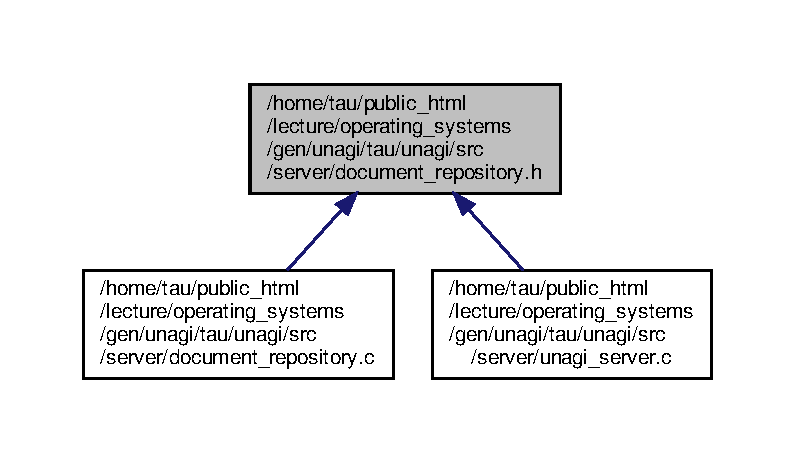
\includegraphics[width=350pt]{document__repository_8h__dep__incl}
\end{center}
\end{figure}
\subsection*{Classes}
\begin{DoxyCompactItemize}
\item 
struct \hyperlink{structdocument__t}{document\+\_\+t}
\begin{DoxyCompactList}\small\item\em 1つのドキュメントを表す構造体(putされる単位) \end{DoxyCompactList}\item 
struct \hyperlink{structdocument__array__t}{document\+\_\+array\+\_\+t}
\begin{DoxyCompactList}\small\item\em ドキュメントの可変長配列 \end{DoxyCompactList}\item 
struct \hyperlink{structdocument__repo__t}{document\+\_\+repo\+\_\+t}
\begin{DoxyCompactList}\small\item\em ドキュメントのレポジトリ \end{DoxyCompactList}\item 
struct \hyperlink{structoccurrence__t}{occurrence\+\_\+t}
\begin{DoxyCompactList}\small\item\em 文書中の検索文字列の出現(occurrence)を表すデータ \end{DoxyCompactList}\item 
struct \hyperlink{structquery__result__t}{query\+\_\+result\+\_\+t}
\begin{DoxyCompactList}\small\item\em 検索結果(出現位置の集合, ストリーム)を表すデータ構造 \end{DoxyCompactList}\item 
struct \hyperlink{structdump__result__t}{dump\+\_\+result\+\_\+t}
\begin{DoxyCompactList}\small\item\em 全ドキュメントのダンプを表すデータ構造 \end{DoxyCompactList}\end{DoxyCompactItemize}
\subsection*{Functions}
\begin{DoxyCompactItemize}
\item 
void \hyperlink{document__repository_8h_ad73236d39e69cbae2e618682cb2faa4e}{document\+\_\+repo\+\_\+init} (\hyperlink{structdocument__repo__t}{document\+\_\+repo\+\_\+t} $\ast$repo)
\begin{DoxyCompactList}\small\item\em ドキュメントレポジトリ(document\+\_\+repo\+\_\+t)の初期化(空にする) \end{DoxyCompactList}\item 
void \hyperlink{document__repository_8h_a3e498b4e62c3223775c173a3b299f412}{document\+\_\+repo\+\_\+destroy} (\hyperlink{structdocument__repo__t}{document\+\_\+repo\+\_\+t} $\ast$repo)
\begin{DoxyCompactList}\small\item\em ドキュメントレポジトリ(document\+\_\+repo\+\_\+t)を破壊する. メモリを開放する \end{DoxyCompactList}\item 
ssize\+\_\+t \hyperlink{document__repository_8h_aa6eebf0d0d4ec7f8d0a79dc7f061502b}{document\+\_\+repo\+\_\+add} (\hyperlink{structdocument__repo__t}{document\+\_\+repo\+\_\+t} $\ast$repo, \hyperlink{structdocument__t}{document\+\_\+t} d)
\begin{DoxyCompactList}\small\item\em ドキュメントレポジトリ(document\+\_\+repo\+\_\+t)にドキュメントを追加する \end{DoxyCompactList}\item 
\hyperlink{structquery__result__t}{query\+\_\+result\+\_\+t} \hyperlink{document__repository_8h_a8f61dbccc6befcc6affb3f6461bff262}{document\+\_\+repo\+\_\+query} (\hyperlink{structdocument__repo__t}{document\+\_\+repo\+\_\+t} $\ast$repo, char $\ast$query, size\+\_\+t query\+\_\+len)
\begin{DoxyCompactList}\small\item\em ドキュメントレポジトリから指定文字列(query)を検索. \end{DoxyCompactList}\item 
\hyperlink{structoccurrence__t}{occurrence\+\_\+t} \hyperlink{document__repository_8h_a7831dbf9173888563e4f19519d700472}{query\+\_\+result\+\_\+next} (\hyperlink{structquery__result__t}{query\+\_\+result\+\_\+t} $\ast$qr)
\begin{DoxyCompactList}\small\item\em document\+\_\+repo\+\_\+query で得られた検索結果から, 次の出現位置を得る \end{DoxyCompactList}\item 
size\+\_\+t \hyperlink{document__repository_8h_a81fe0bb9c8482bbaa25b277dbf1a22ad}{document\+\_\+repo\+\_\+queryc} (\hyperlink{structdocument__repo__t}{document\+\_\+repo\+\_\+t} $\ast$repo, char $\ast$query, size\+\_\+t query\+\_\+len)
\begin{DoxyCompactList}\small\item\em ドキュメントレポジトリから指定文字列(query)を検索しその出現回数 (のみ)を返す \end{DoxyCompactList}\item 
\hyperlink{structdump__result__t}{dump\+\_\+result\+\_\+t} \hyperlink{document__repository_8h_a668ef0ea9ec3a0ca0bcb98b2406eb477}{document\+\_\+repo\+\_\+dump} (\hyperlink{structdocument__repo__t}{document\+\_\+repo\+\_\+t} $\ast$repo)
\begin{DoxyCompactList}\small\item\em 全ドキュメントのダンプを表すデータ構造 \end{DoxyCompactList}\item 
\mbox{\Hypertarget{document__repository_8h_affebc850b20de4382fff4a039f59c5a7}\label{document__repository_8h_affebc850b20de4382fff4a039f59c5a7}} 
size\+\_\+t \hyperlink{document__repository_8h_affebc850b20de4382fff4a039f59c5a7}{document\+\_\+repo\+\_\+n\+\_\+docs} (\hyperlink{structdocument__repo__t}{document\+\_\+repo\+\_\+t} $\ast$repo)
\begin{DoxyCompactList}\small\item\em 全ドキュメント数を取得する. \end{DoxyCompactList}\item 
\mbox{\Hypertarget{document__repository_8h_a2db0fd4b412e33d8bf3549feb98b22fb}\label{document__repository_8h_a2db0fd4b412e33d8bf3549feb98b22fb}} 
\hyperlink{structdocument__t}{document\+\_\+t} \hyperlink{document__repository_8h_a2db0fd4b412e33d8bf3549feb98b22fb}{dump\+\_\+result\+\_\+next} (\hyperlink{structdump__result__t}{dump\+\_\+result\+\_\+t} $\ast$dr)
\begin{DoxyCompactList}\small\item\em document\+\_\+repo\+\_\+dump が返した \hyperlink{structdump__result__t}{dump\+\_\+result\+\_\+t} から, 次のドキュメントを返す. \end{DoxyCompactList}\end{DoxyCompactItemize}


\subsection{Detailed Description}
ドキュメントを登録, 検索するレポジトリ(ヘッダファイル) 

\begin{DoxyAuthor}{Author}
田浦 
\end{DoxyAuthor}
\begin{DoxyDate}{Date}
Oct. 8, 2018 
\end{DoxyDate}


\subsection{Function Documentation}
\mbox{\Hypertarget{document__repository_8h_aa6eebf0d0d4ec7f8d0a79dc7f061502b}\label{document__repository_8h_aa6eebf0d0d4ec7f8d0a79dc7f061502b}} 
\index{document\+\_\+repository.\+h@{document\+\_\+repository.\+h}!document\+\_\+repo\+\_\+add@{document\+\_\+repo\+\_\+add}}
\index{document\+\_\+repo\+\_\+add@{document\+\_\+repo\+\_\+add}!document\+\_\+repository.\+h@{document\+\_\+repository.\+h}}
\subsubsection{\texorpdfstring{document\+\_\+repo\+\_\+add()}{document\_repo\_add()}}
{\footnotesize\ttfamily ssize\+\_\+t document\+\_\+repo\+\_\+add (\begin{DoxyParamCaption}\item[{\hyperlink{structdocument__repo__t}{document\+\_\+repo\+\_\+t} $\ast$}]{repo,  }\item[{\hyperlink{structdocument__t}{document\+\_\+t}}]{d }\end{DoxyParamCaption})}



ドキュメントレポジトリ(document\+\_\+repo\+\_\+t)にドキュメントを追加する 

\begin{DoxyReturn}{Returns}
成功したら, 非負の整数. 失敗(メモリ割り当て失敗)したら-\/1.
\end{DoxyReturn}
\begin{DoxySeeAlso}{See also}
\hyperlink{document__repository_8c_ad73236d39e69cbae2e618682cb2faa4e}{document\+\_\+repo\+\_\+init} 

\hyperlink{document__repository_8c_a3e498b4e62c3223775c173a3b299f412}{document\+\_\+repo\+\_\+destroy} 

\hyperlink{structdocument__repo__t}{document\+\_\+repo\+\_\+t} 
\end{DoxySeeAlso}
\mbox{\Hypertarget{document__repository_8h_a3e498b4e62c3223775c173a3b299f412}\label{document__repository_8h_a3e498b4e62c3223775c173a3b299f412}} 
\index{document\+\_\+repository.\+h@{document\+\_\+repository.\+h}!document\+\_\+repo\+\_\+destroy@{document\+\_\+repo\+\_\+destroy}}
\index{document\+\_\+repo\+\_\+destroy@{document\+\_\+repo\+\_\+destroy}!document\+\_\+repository.\+h@{document\+\_\+repository.\+h}}
\subsubsection{\texorpdfstring{document\+\_\+repo\+\_\+destroy()}{document\_repo\_destroy()}}
{\footnotesize\ttfamily void document\+\_\+repo\+\_\+destroy (\begin{DoxyParamCaption}\item[{\hyperlink{structdocument__repo__t}{document\+\_\+repo\+\_\+t} $\ast$}]{repo }\end{DoxyParamCaption})}



ドキュメントレポジトリ(document\+\_\+repo\+\_\+t)を破壊する. メモリを開放する 

\begin{DoxySeeAlso}{See also}
\hyperlink{document__repository_8c_ad73236d39e69cbae2e618682cb2faa4e}{document\+\_\+repo\+\_\+init} 

\hyperlink{document__repository_8c_aa6eebf0d0d4ec7f8d0a79dc7f061502b}{document\+\_\+repo\+\_\+add} 

\hyperlink{structdocument__repo__t}{document\+\_\+repo\+\_\+t} 
\end{DoxySeeAlso}
\mbox{\Hypertarget{document__repository_8h_a668ef0ea9ec3a0ca0bcb98b2406eb477}\label{document__repository_8h_a668ef0ea9ec3a0ca0bcb98b2406eb477}} 
\index{document\+\_\+repository.\+h@{document\+\_\+repository.\+h}!document\+\_\+repo\+\_\+dump@{document\+\_\+repo\+\_\+dump}}
\index{document\+\_\+repo\+\_\+dump@{document\+\_\+repo\+\_\+dump}!document\+\_\+repository.\+h@{document\+\_\+repository.\+h}}
\subsubsection{\texorpdfstring{document\+\_\+repo\+\_\+dump()}{document\_repo\_dump()}}
{\footnotesize\ttfamily \hyperlink{structdump__result__t}{dump\+\_\+result\+\_\+t} document\+\_\+repo\+\_\+dump (\begin{DoxyParamCaption}\item[{\hyperlink{structdocument__repo__t}{document\+\_\+repo\+\_\+t} $\ast$}]{repo }\end{DoxyParamCaption})}



全ドキュメントのダンプを表すデータ構造 

\begin{DoxySeeAlso}{See also}
\hyperlink{document__repository_8c_a668ef0ea9ec3a0ca0bcb98b2406eb477}{document\+\_\+repo\+\_\+dump} 

\hyperlink{document__repository_8c_a2db0fd4b412e33d8bf3549feb98b22fb}{dump\+\_\+result\+\_\+next}
\end{DoxySeeAlso}
一般に全ドキュメントは大量になりうるため, ドキュメントダンプの結果は, ドキュメントを一つずつ返すことができる データ構造とする. 具体的には, dump\+\_\+result\+\_\+next という関数で, 次のドキュメントを返すようなデータ構造とする. 従って以下のように使う.

\hyperlink{structdump__result__t}{dump\+\_\+result\+\_\+t} qr = document\+\_\+repo\+\_\+dump(repo);

while (1) \{

\hyperlink{structdocument__t}{document\+\_\+t} doc = dump\+\_\+result\+\_\+next(\&qr);

if (!doc.label) break;

... doc.\+data ...

\} 全ドキュメントのダンプを取得する

\hyperlink{structdump__result__t}{dump\+\_\+result\+\_\+t} 型の構造体を返す. その構造体は, dump\+\_\+result\+\_\+next(..) 関数を次々と呼ぶことで, 次々に ドキュメントを返す. \mbox{\Hypertarget{document__repository_8h_ad73236d39e69cbae2e618682cb2faa4e}\label{document__repository_8h_ad73236d39e69cbae2e618682cb2faa4e}} 
\index{document\+\_\+repository.\+h@{document\+\_\+repository.\+h}!document\+\_\+repo\+\_\+init@{document\+\_\+repo\+\_\+init}}
\index{document\+\_\+repo\+\_\+init@{document\+\_\+repo\+\_\+init}!document\+\_\+repository.\+h@{document\+\_\+repository.\+h}}
\subsubsection{\texorpdfstring{document\+\_\+repo\+\_\+init()}{document\_repo\_init()}}
{\footnotesize\ttfamily void document\+\_\+repo\+\_\+init (\begin{DoxyParamCaption}\item[{\hyperlink{structdocument__repo__t}{document\+\_\+repo\+\_\+t} $\ast$}]{repo }\end{DoxyParamCaption})}



ドキュメントレポジトリ(document\+\_\+repo\+\_\+t)の初期化(空にする) 

\begin{DoxySeeAlso}{See also}
\hyperlink{document__repository_8c_a3e498b4e62c3223775c173a3b299f412}{document\+\_\+repo\+\_\+destroy} 

\hyperlink{document__repository_8c_aa6eebf0d0d4ec7f8d0a79dc7f061502b}{document\+\_\+repo\+\_\+add} 

\hyperlink{structdocument__repo__t}{document\+\_\+repo\+\_\+t} 
\end{DoxySeeAlso}
\mbox{\Hypertarget{document__repository_8h_a8f61dbccc6befcc6affb3f6461bff262}\label{document__repository_8h_a8f61dbccc6befcc6affb3f6461bff262}} 
\index{document\+\_\+repository.\+h@{document\+\_\+repository.\+h}!document\+\_\+repo\+\_\+query@{document\+\_\+repo\+\_\+query}}
\index{document\+\_\+repo\+\_\+query@{document\+\_\+repo\+\_\+query}!document\+\_\+repository.\+h@{document\+\_\+repository.\+h}}
\subsubsection{\texorpdfstring{document\+\_\+repo\+\_\+query()}{document\_repo\_query()}}
{\footnotesize\ttfamily \hyperlink{structquery__result__t}{query\+\_\+result\+\_\+t} document\+\_\+repo\+\_\+query (\begin{DoxyParamCaption}\item[{\hyperlink{structdocument__repo__t}{document\+\_\+repo\+\_\+t} $\ast$}]{repo,  }\item[{char $\ast$}]{query,  }\item[{size\+\_\+t}]{query\+\_\+len }\end{DoxyParamCaption})}



ドキュメントレポジトリから指定文字列(query)を検索. 

\begin{DoxyReturn}{Returns}
検索結果(query\+\_\+result\+\_\+t) 
\end{DoxyReturn}
\begin{DoxySeeAlso}{See also}
\hyperlink{structquery__result__t}{query\+\_\+result\+\_\+t} 

\hyperlink{document__repository_8c_a7831dbf9173888563e4f19519d700472}{query\+\_\+result\+\_\+next} 

\hyperlink{document__repository_8c_aa6eebf0d0d4ec7f8d0a79dc7f061502b}{document\+\_\+repo\+\_\+add}
\end{DoxySeeAlso}
ドキュメントレポジトリ内の全ドキュメント(これまでに document\+\_\+repo\+\_\+add されたすべてのドキュメント)から検索文字列 query の出現を検索する. query\+\_\+result\+\_\+next は, そこから全ての出現位置を取 得することができるようなデータである. 詳しくは, \hyperlink{structquery__result__t}{query\+\_\+result\+\_\+t} のド キュメントを参照 
\begin{DoxyParams}{Parameters}
{\em repo} & 検索対象のドキュメントレポジトリ \\
\hline
{\em query} & 検索文字列 \\
\hline
{\em query\+\_\+len} & queryの長さ(バイト数) \\
\hline
\end{DoxyParams}
\mbox{\Hypertarget{document__repository_8h_a81fe0bb9c8482bbaa25b277dbf1a22ad}\label{document__repository_8h_a81fe0bb9c8482bbaa25b277dbf1a22ad}} 
\index{document\+\_\+repository.\+h@{document\+\_\+repository.\+h}!document\+\_\+repo\+\_\+queryc@{document\+\_\+repo\+\_\+queryc}}
\index{document\+\_\+repo\+\_\+queryc@{document\+\_\+repo\+\_\+queryc}!document\+\_\+repository.\+h@{document\+\_\+repository.\+h}}
\subsubsection{\texorpdfstring{document\+\_\+repo\+\_\+queryc()}{document\_repo\_queryc()}}
{\footnotesize\ttfamily size\+\_\+t document\+\_\+repo\+\_\+queryc (\begin{DoxyParamCaption}\item[{\hyperlink{structdocument__repo__t}{document\+\_\+repo\+\_\+t} $\ast$}]{repo,  }\item[{char $\ast$}]{query,  }\item[{size\+\_\+t}]{query\+\_\+len }\end{DoxyParamCaption})}



ドキュメントレポジトリから指定文字列(query)を検索しその出現回数 (のみ)を返す 

\begin{DoxyReturn}{Returns}
出現回数 
\end{DoxyReturn}
\begin{DoxySeeAlso}{See also}
\hyperlink{structquery__result__t}{query\+\_\+result\+\_\+t} 

\hyperlink{document__repository_8c_a7831dbf9173888563e4f19519d700472}{query\+\_\+result\+\_\+next} 

\hyperlink{document__repository_8c_a8f61dbccc6befcc6affb3f6461bff262}{document\+\_\+repo\+\_\+query} 

\hyperlink{document__repository_8c_aa6eebf0d0d4ec7f8d0a79dc7f061502b}{document\+\_\+repo\+\_\+add}
\end{DoxySeeAlso}
ドキュメントレポジトリ内の全ドキュメント(これまでに document\+\_\+repo\+\_\+add されたすべてのドキュメント)から検索文字列 query の出現を検索する. query\+\_\+result\+\_\+next は, そこから全ての出現位置を取 得することができるようなデータである. 詳しくは, \hyperlink{structquery__result__t}{query\+\_\+result\+\_\+t} のド キュメントを参照 
\begin{DoxyParams}{Parameters}
{\em repo} & 検索対象のドキュメントレポジトリ \\
\hline
{\em query} & 検索文字列 \\
\hline
{\em query\+\_\+len} & queryの長さ(バイト数) \\
\hline
\end{DoxyParams}
\mbox{\Hypertarget{document__repository_8h_a7831dbf9173888563e4f19519d700472}\label{document__repository_8h_a7831dbf9173888563e4f19519d700472}} 
\index{document\+\_\+repository.\+h@{document\+\_\+repository.\+h}!query\+\_\+result\+\_\+next@{query\+\_\+result\+\_\+next}}
\index{query\+\_\+result\+\_\+next@{query\+\_\+result\+\_\+next}!document\+\_\+repository.\+h@{document\+\_\+repository.\+h}}
\subsubsection{\texorpdfstring{query\+\_\+result\+\_\+next()}{query\_result\_next()}}
{\footnotesize\ttfamily \hyperlink{structoccurrence__t}{occurrence\+\_\+t} query\+\_\+result\+\_\+next (\begin{DoxyParamCaption}\item[{\hyperlink{structquery__result__t}{query\+\_\+result\+\_\+t} $\ast$}]{qr }\end{DoxyParamCaption})}



document\+\_\+repo\+\_\+query で得られた検索結果から, 次の出現位置を得る 

\begin{DoxyReturn}{Returns}
検索文字列の次の出現位置(occurrence\+\_\+t)
\end{DoxyReturn}
\begin{DoxySeeAlso}{See also}
\hyperlink{document__repository_8c_a8f61dbccc6befcc6affb3f6461bff262}{document\+\_\+repo\+\_\+query} 

\hyperlink{structquery__result__t}{query\+\_\+result\+\_\+t}
\end{DoxySeeAlso}
document\+\_\+repo\+\_\+query が返した「検索結果(\hyperlink{structquery__result__t}{query\+\_\+result\+\_\+t} 型の データ)」から, 検索文字列の「次の」出現位置を得る. 検索結果に対して この関数を次々と呼び出すことで, すべての出現位置を得ることができる. document\+\_\+repo\+\_\+query 現在の検索アルゴリズムは非常に単純(非効率)なも ので, (putで)蓄えられたドキュメントを順に, スキャンしていくだけのも の. ひとつのドキュメントから文字列を検索するには\+Cのstrstr 関数を 呼ぶ(man strstr して調べよ). 
\begin{DoxyParams}{Parameters}
{\em qr} & document\+\_\+repo\+\_\+queryが返した検索結果 \\
\hline
\end{DoxyParams}

\hypertarget{unagi__server_8c}{}\section{/home/tau/public\+\_\+html/lecture/operating\+\_\+systems/gen/unagi/tau/unagi/src/server/unagi\+\_\+server.c File Reference}
\label{unagi__server_8c}\index{/home/tau/public\+\_\+html/lecture/operating\+\_\+systems/gen/unagi/tau/unagi/src/server/unagi\+\_\+server.\+c@{/home/tau/public\+\_\+html/lecture/operating\+\_\+systems/gen/unagi/tau/unagi/src/server/unagi\+\_\+server.\+c}}


unagi server メインファイル  


{\ttfamily \#include $<$assert.\+h$>$}\newline
{\ttfamily \#include $<$ctype.\+h$>$}\newline
{\ttfamily \#include $<$stdio.\+h$>$}\newline
{\ttfamily \#include $<$stdlib.\+h$>$}\newline
{\ttfamily \#include $<$string.\+h$>$}\newline
{\ttfamily \#include $<$sys/socket.\+h$>$}\newline
{\ttfamily \#include $<$netinet/in.\+h$>$}\newline
{\ttfamily \#include $<$netinet/tcp.\+h$>$}\newline
{\ttfamily \#include $<$sys/types.\+h$>$}\newline
{\ttfamily \#include $<$arpa/inet.\+h$>$}\newline
{\ttfamily \#include $<$unistd.\+h$>$}\newline
{\ttfamily \#include \char`\"{}unagi\+\_\+utility.\+h\char`\"{}}\newline
{\ttfamily \#include \char`\"{}document\+\_\+repository.\+h\char`\"{}}\newline
Include dependency graph for unagi\+\_\+server.\+c\+:\nopagebreak
\begin{figure}[H]
\begin{center}
\leavevmode
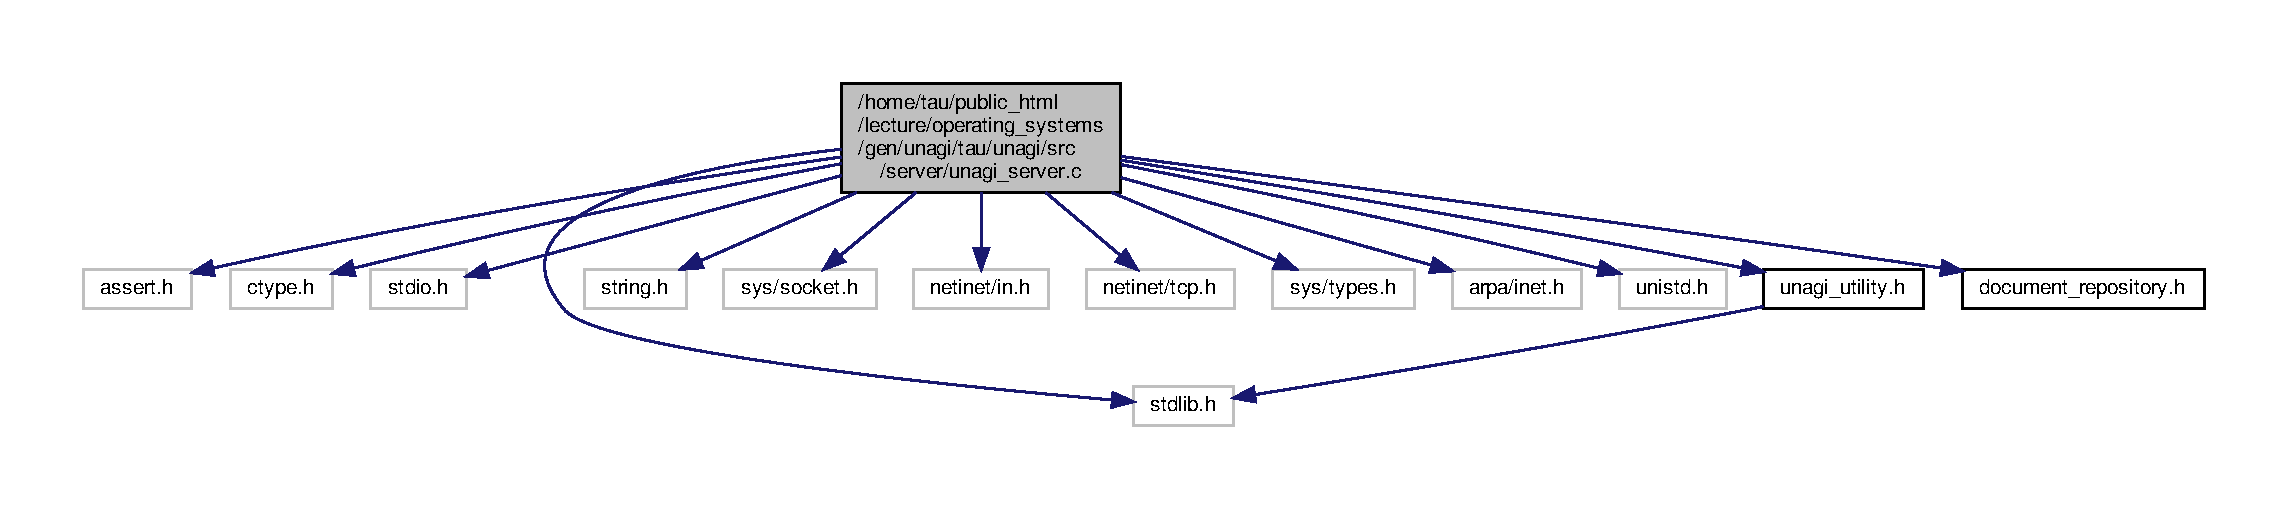
\includegraphics[width=350pt]{unagi__server_8c__incl}
\end{center}
\end{figure}
\subsection*{Classes}
\begin{DoxyCompactItemize}
\item 
struct \hyperlink{structcmdline__options__t}{cmdline\+\_\+options\+\_\+t}
\begin{DoxyCompactList}\small\item\em サーバのコマンドラインオプションを表すデータ構造 \end{DoxyCompactList}\item 
struct \hyperlink{structserver__t}{server\+\_\+t}
\begin{DoxyCompactList}\small\item\em サーバを表すデータ構造 \end{DoxyCompactList}\item 
struct \hyperlink{structrequest__t}{request\+\_\+t}
\begin{DoxyCompactList}\small\item\em クライアントからのリクエストを表すデータ構造 \end{DoxyCompactList}\end{DoxyCompactItemize}
\subsection*{Macros}
\begin{DoxyCompactItemize}
\item 
\mbox{\Hypertarget{unagi__server_8c_a5f07c7dadef9a7101111edab4f7ad98d}\label{unagi__server_8c_a5f07c7dadef9a7101111edab4f7ad98d}} 
\#define \hyperlink{unagi__server_8c_a5f07c7dadef9a7101111edab4f7ad98d}{options\+\_\+default\+\_\+port}~0
\begin{DoxyCompactList}\small\item\em デフォルトのポート番号(0 \+: O\+Sに選ばせる) \end{DoxyCompactList}\item 
\mbox{\Hypertarget{unagi__server_8c_a76204a4a1bf3968aee3a7af2c09d6b70}\label{unagi__server_8c_a76204a4a1bf3968aee3a7af2c09d6b70}} 
\#define \hyperlink{unagi__server_8c_a76204a4a1bf3968aee3a7af2c09d6b70}{options\+\_\+default\+\_\+qlen}~1000
\begin{DoxyCompactList}\small\item\em デフォルトの接続待ちキュー \end{DoxyCompactList}\item 
\mbox{\Hypertarget{unagi__server_8c_ae757f1a505785321d99a471883df9541}\label{unagi__server_8c_ae757f1a505785321d99a471883df9541}} 
\#define \hyperlink{unagi__server_8c_ae757f1a505785321d99a471883df9541}{options\+\_\+default\+\_\+log}~\char`\"{}unagi.\+log\char`\"{}
\begin{DoxyCompactList}\small\item\em デフォルトのログファイル名 \end{DoxyCompactList}\end{DoxyCompactItemize}
\subsection*{Enumerations}
\begin{DoxyCompactItemize}
\item 
enum \hyperlink{unagi__server_8c_a30a7f6ee9120da0c95e8a1847b35a7a2}{request\+\_\+kind\+\_\+t} \{ \newline
\hyperlink{unagi__server_8c_a30a7f6ee9120da0c95e8a1847b35a7a2a939edab734abb6b3618470014284c9bb}{request\+\_\+kind\+\_\+put}, 
\hyperlink{unagi__server_8c_a30a7f6ee9120da0c95e8a1847b35a7a2a3b425dde6f4f1c9af3b7364789a7861a}{request\+\_\+kind\+\_\+get}, 
\hyperlink{unagi__server_8c_a30a7f6ee9120da0c95e8a1847b35a7a2a561c4bcc9e55396b0f97b4689b858cce}{request\+\_\+kind\+\_\+getc}, 
\hyperlink{unagi__server_8c_a30a7f6ee9120da0c95e8a1847b35a7a2add50a1ff1f7fed7f2d79766a99661650}{request\+\_\+kind\+\_\+dump}, 
\newline
\hyperlink{unagi__server_8c_a30a7f6ee9120da0c95e8a1847b35a7a2a03dcc800e7750f6b6738b7e8cfbf175d}{request\+\_\+kind\+\_\+dumpc}, 
\hyperlink{unagi__server_8c_a30a7f6ee9120da0c95e8a1847b35a7a2afc515b19b1b933e6ba491cc96528bdae}{request\+\_\+kind\+\_\+discon}, 
\hyperlink{unagi__server_8c_a30a7f6ee9120da0c95e8a1847b35a7a2a8d686e8fb6bb9044d4c36920e5c6f442}{request\+\_\+kind\+\_\+quit}, 
\hyperlink{unagi__server_8c_a30a7f6ee9120da0c95e8a1847b35a7a2a4d0a6943b5e744685646ad25c21e24f2}{request\+\_\+kind\+\_\+invalid}
 \}\begin{DoxyCompactList}\small\item\em クライアントからのリクエストの種類 \end{DoxyCompactList}
\end{DoxyCompactItemize}
\subsection*{Functions}
\begin{DoxyCompactItemize}
\item 
int \hyperlink{unagi__server_8c_a3c04138a5bfe5d72780bb7e82a18e627}{main} (int argc, char $\ast$$\ast$argv)
\begin{DoxyCompactList}\small\item\em メイン関数 \end{DoxyCompactList}\end{DoxyCompactItemize}
\subsection*{Variables}
\begin{DoxyCompactItemize}
\item 
const int \hyperlink{unagi__server_8c_a212b47c04ff57543a47a8d70f841c9db}{max\+\_\+inst\+\_\+len} = 20
\item 
const int \hyperlink{unagi__server_8c_a964cb5d8e42b8e8d6075b23e01bdaf36}{max\+\_\+num\+\_\+len} = 20
\end{DoxyCompactItemize}


\subsection{Detailed Description}
unagi server メインファイル 

\begin{DoxyAuthor}{Author}
田浦 
\end{DoxyAuthor}
\begin{DoxyDate}{Date}
Oct. 8, 2018 
\end{DoxyDate}


\subsection{Enumeration Type Documentation}
\mbox{\Hypertarget{unagi__server_8c_a30a7f6ee9120da0c95e8a1847b35a7a2}\label{unagi__server_8c_a30a7f6ee9120da0c95e8a1847b35a7a2}} 
\index{unagi\+\_\+server.\+c@{unagi\+\_\+server.\+c}!request\+\_\+kind\+\_\+t@{request\+\_\+kind\+\_\+t}}
\index{request\+\_\+kind\+\_\+t@{request\+\_\+kind\+\_\+t}!unagi\+\_\+server.\+c@{unagi\+\_\+server.\+c}}
\subsubsection{\texorpdfstring{request\+\_\+kind\+\_\+t}{request\_kind\_t}}
{\footnotesize\ttfamily enum \hyperlink{unagi__server_8c_a30a7f6ee9120da0c95e8a1847b35a7a2}{request\+\_\+kind\+\_\+t}}



クライアントからのリクエストの種類 

\begin{DoxyEnumFields}{Enumerator}
\raisebox{\heightof{T}}[0pt][0pt]{\index{request\+\_\+kind\+\_\+put@{request\+\_\+kind\+\_\+put}!unagi\+\_\+server.\+c@{unagi\+\_\+server.\+c}}\index{unagi\+\_\+server.\+c@{unagi\+\_\+server.\+c}!request\+\_\+kind\+\_\+put@{request\+\_\+kind\+\_\+put}}}\mbox{\Hypertarget{unagi__server_8c_a30a7f6ee9120da0c95e8a1847b35a7a2a939edab734abb6b3618470014284c9bb}\label{unagi__server_8c_a30a7f6ee9120da0c95e8a1847b35a7a2a939edab734abb6b3618470014284c9bb}} 
request\+\_\+kind\+\_\+put&put (ドキュメント追加) \\
\hline

\raisebox{\heightof{T}}[0pt][0pt]{\index{request\+\_\+kind\+\_\+get@{request\+\_\+kind\+\_\+get}!unagi\+\_\+server.\+c@{unagi\+\_\+server.\+c}}\index{unagi\+\_\+server.\+c@{unagi\+\_\+server.\+c}!request\+\_\+kind\+\_\+get@{request\+\_\+kind\+\_\+get}}}\mbox{\Hypertarget{unagi__server_8c_a30a7f6ee9120da0c95e8a1847b35a7a2a3b425dde6f4f1c9af3b7364789a7861a}\label{unagi__server_8c_a30a7f6ee9120da0c95e8a1847b35a7a2a3b425dde6f4f1c9af3b7364789a7861a}} 
request\+\_\+kind\+\_\+get&get (文字列検索) \\
\hline

\raisebox{\heightof{T}}[0pt][0pt]{\index{request\+\_\+kind\+\_\+getc@{request\+\_\+kind\+\_\+getc}!unagi\+\_\+server.\+c@{unagi\+\_\+server.\+c}}\index{unagi\+\_\+server.\+c@{unagi\+\_\+server.\+c}!request\+\_\+kind\+\_\+getc@{request\+\_\+kind\+\_\+getc}}}\mbox{\Hypertarget{unagi__server_8c_a30a7f6ee9120da0c95e8a1847b35a7a2a561c4bcc9e55396b0f97b4689b858cce}\label{unagi__server_8c_a30a7f6ee9120da0c95e8a1847b35a7a2a561c4bcc9e55396b0f97b4689b858cce}} 
request\+\_\+kind\+\_\+getc&getc (文字列出現数) \\
\hline

\raisebox{\heightof{T}}[0pt][0pt]{\index{request\+\_\+kind\+\_\+dump@{request\+\_\+kind\+\_\+dump}!unagi\+\_\+server.\+c@{unagi\+\_\+server.\+c}}\index{unagi\+\_\+server.\+c@{unagi\+\_\+server.\+c}!request\+\_\+kind\+\_\+dump@{request\+\_\+kind\+\_\+dump}}}\mbox{\Hypertarget{unagi__server_8c_a30a7f6ee9120da0c95e8a1847b35a7a2add50a1ff1f7fed7f2d79766a99661650}\label{unagi__server_8c_a30a7f6ee9120da0c95e8a1847b35a7a2add50a1ff1f7fed7f2d79766a99661650}} 
request\+\_\+kind\+\_\+dump&dump (全ドキュメントダンプ) \\
\hline

\raisebox{\heightof{T}}[0pt][0pt]{\index{request\+\_\+kind\+\_\+dumpc@{request\+\_\+kind\+\_\+dumpc}!unagi\+\_\+server.\+c@{unagi\+\_\+server.\+c}}\index{unagi\+\_\+server.\+c@{unagi\+\_\+server.\+c}!request\+\_\+kind\+\_\+dumpc@{request\+\_\+kind\+\_\+dumpc}}}\mbox{\Hypertarget{unagi__server_8c_a30a7f6ee9120da0c95e8a1847b35a7a2a03dcc800e7750f6b6738b7e8cfbf175d}\label{unagi__server_8c_a30a7f6ee9120da0c95e8a1847b35a7a2a03dcc800e7750f6b6738b7e8cfbf175d}} 
request\+\_\+kind\+\_\+dumpc&dumpc (全ドキュメント数) \\
\hline

\raisebox{\heightof{T}}[0pt][0pt]{\index{request\+\_\+kind\+\_\+discon@{request\+\_\+kind\+\_\+discon}!unagi\+\_\+server.\+c@{unagi\+\_\+server.\+c}}\index{unagi\+\_\+server.\+c@{unagi\+\_\+server.\+c}!request\+\_\+kind\+\_\+discon@{request\+\_\+kind\+\_\+discon}}}\mbox{\Hypertarget{unagi__server_8c_a30a7f6ee9120da0c95e8a1847b35a7a2afc515b19b1b933e6ba491cc96528bdae}\label{unagi__server_8c_a30a7f6ee9120da0c95e8a1847b35a7a2afc515b19b1b933e6ba491cc96528bdae}} 
request\+\_\+kind\+\_\+discon&discon (接続終了) \\
\hline

\raisebox{\heightof{T}}[0pt][0pt]{\index{request\+\_\+kind\+\_\+quit@{request\+\_\+kind\+\_\+quit}!unagi\+\_\+server.\+c@{unagi\+\_\+server.\+c}}\index{unagi\+\_\+server.\+c@{unagi\+\_\+server.\+c}!request\+\_\+kind\+\_\+quit@{request\+\_\+kind\+\_\+quit}}}\mbox{\Hypertarget{unagi__server_8c_a30a7f6ee9120da0c95e8a1847b35a7a2a8d686e8fb6bb9044d4c36920e5c6f442}\label{unagi__server_8c_a30a7f6ee9120da0c95e8a1847b35a7a2a8d686e8fb6bb9044d4c36920e5c6f442}} 
request\+\_\+kind\+\_\+quit&quit (サーバ終了) \\
\hline

\raisebox{\heightof{T}}[0pt][0pt]{\index{request\+\_\+kind\+\_\+invalid@{request\+\_\+kind\+\_\+invalid}!unagi\+\_\+server.\+c@{unagi\+\_\+server.\+c}}\index{unagi\+\_\+server.\+c@{unagi\+\_\+server.\+c}!request\+\_\+kind\+\_\+invalid@{request\+\_\+kind\+\_\+invalid}}}\mbox{\Hypertarget{unagi__server_8c_a30a7f6ee9120da0c95e8a1847b35a7a2a4d0a6943b5e744685646ad25c21e24f2}\label{unagi__server_8c_a30a7f6ee9120da0c95e8a1847b35a7a2a4d0a6943b5e744685646ad25c21e24f2}} 
request\+\_\+kind\+\_\+invalid&無効なリクエスト \\
\hline

\end{DoxyEnumFields}


\subsection{Function Documentation}
\mbox{\Hypertarget{unagi__server_8c_a3c04138a5bfe5d72780bb7e82a18e627}\label{unagi__server_8c_a3c04138a5bfe5d72780bb7e82a18e627}} 
\index{unagi\+\_\+server.\+c@{unagi\+\_\+server.\+c}!main@{main}}
\index{main@{main}!unagi\+\_\+server.\+c@{unagi\+\_\+server.\+c}}
\subsubsection{\texorpdfstring{main()}{main()}}
{\footnotesize\ttfamily int main (\begin{DoxyParamCaption}\item[{int}]{argc,  }\item[{char $\ast$$\ast$}]{argv }\end{DoxyParamCaption})}



メイン関数 

コマンドラインを処理. サーバを立ち上げ. 停止(quit)命令を受け取るまで処理を 

\subsection{Variable Documentation}
\mbox{\Hypertarget{unagi__server_8c_a212b47c04ff57543a47a8d70f841c9db}\label{unagi__server_8c_a212b47c04ff57543a47a8d70f841c9db}} 
\index{unagi\+\_\+server.\+c@{unagi\+\_\+server.\+c}!max\+\_\+inst\+\_\+len@{max\+\_\+inst\+\_\+len}}
\index{max\+\_\+inst\+\_\+len@{max\+\_\+inst\+\_\+len}!unagi\+\_\+server.\+c@{unagi\+\_\+server.\+c}}
\subsubsection{\texorpdfstring{max\+\_\+inst\+\_\+len}{max\_inst\_len}}
{\footnotesize\ttfamily const int max\+\_\+inst\+\_\+len = 20}

命令(put, get, quit, ...)の最大長 \mbox{\Hypertarget{unagi__server_8c_a964cb5d8e42b8e8d6075b23e01bdaf36}\label{unagi__server_8c_a964cb5d8e42b8e8d6075b23e01bdaf36}} 
\index{unagi\+\_\+server.\+c@{unagi\+\_\+server.\+c}!max\+\_\+num\+\_\+len@{max\+\_\+num\+\_\+len}}
\index{max\+\_\+num\+\_\+len@{max\+\_\+num\+\_\+len}!unagi\+\_\+server.\+c@{unagi\+\_\+server.\+c}}
\subsubsection{\texorpdfstring{max\+\_\+num\+\_\+len}{max\_num\_len}}
{\footnotesize\ttfamily const int max\+\_\+num\+\_\+len = 20}

数字の最大桁数 
\hypertarget{unagi__utility_8c}{}\section{/home/tau/public\+\_\+html/lecture/operating\+\_\+systems/gen/unagi/tau/unagi/src/server/unagi\+\_\+utility.c File Reference}
\label{unagi__utility_8c}\index{/home/tau/public\+\_\+html/lecture/operating\+\_\+systems/gen/unagi/tau/unagi/src/server/unagi\+\_\+utility.\+c@{/home/tau/public\+\_\+html/lecture/operating\+\_\+systems/gen/unagi/tau/unagi/src/server/unagi\+\_\+utility.\+c}}


共通に使うユーティリティ  


{\ttfamily \#include $<$stdio.\+h$>$}\newline
{\ttfamily \#include \char`\"{}unagi\+\_\+utility.\+h\char`\"{}}\newline
Include dependency graph for unagi\+\_\+utility.\+c\+:\nopagebreak
\begin{figure}[H]
\begin{center}
\leavevmode
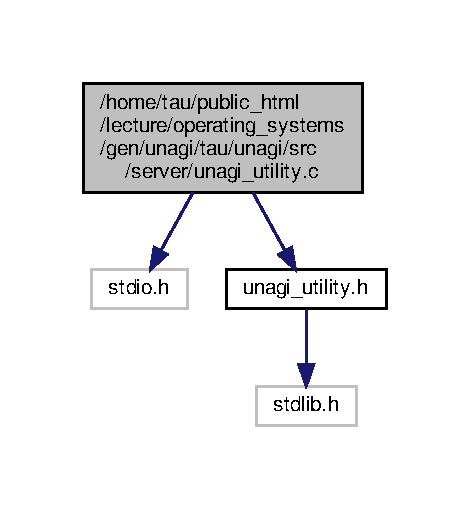
\includegraphics[width=226pt]{unagi__utility_8c__incl}
\end{center}
\end{figure}
\subsection*{Functions}
\begin{DoxyCompactItemize}
\item 
void \hyperlink{unagi__utility_8c_a6f52d6a6178c8fbb9e4393d00911c6b5}{api\+\_\+err\+\_\+} (const char $\ast$msg, const char $\ast$\+\_\+\+\_\+file\+\_\+\+\_\+, int \+\_\+\+\_\+line\+\_\+\+\_\+)
\begin{DoxyCompactList}\small\item\em マクロ api\+\_\+err を参照 \end{DoxyCompactList}\item 
void \hyperlink{unagi__utility_8c_aa728038408058b42e2a43e01722cbd49}{internal\+\_\+err\+\_\+} (const char $\ast$msg, const char $\ast$\+\_\+\+\_\+file\+\_\+\+\_\+, int \+\_\+\+\_\+line\+\_\+\+\_\+)
\begin{DoxyCompactList}\small\item\em マクロ internal\+\_\+err を参照 \end{DoxyCompactList}\item 
void $\ast$ \hyperlink{unagi__utility_8c_a7f6cb815cae2536139cd0315633f713b}{malloc\+\_\+or\+\_\+err} (size\+\_\+t sz)
\begin{DoxyCompactList}\small\item\em mallocし, 失敗したらエラーを表示 \end{DoxyCompactList}\item 
\mbox{\Hypertarget{unagi__utility_8c_ad7a4504082a1eeca5b70e47273d3af6b}\label{unagi__utility_8c_ad7a4504082a1eeca5b70e47273d3af6b}} 
void \hyperlink{unagi__utility_8c_ad7a4504082a1eeca5b70e47273d3af6b}{my\+\_\+free} (void $\ast$a)
\begin{DoxyCompactList}\small\item\em freeの代わりにこれを呼ぶ \end{DoxyCompactList}\end{DoxyCompactItemize}


\subsection{Detailed Description}
共通に使うユーティリティ 

\begin{DoxyAuthor}{Author}
田浦 
\end{DoxyAuthor}
\begin{DoxyDate}{Date}
Oct. 8, 2018 
\end{DoxyDate}


\subsection{Function Documentation}
\mbox{\Hypertarget{unagi__utility_8c_a6f52d6a6178c8fbb9e4393d00911c6b5}\label{unagi__utility_8c_a6f52d6a6178c8fbb9e4393d00911c6b5}} 
\index{unagi\+\_\+utility.\+c@{unagi\+\_\+utility.\+c}!api\+\_\+err\+\_\+@{api\+\_\+err\+\_\+}}
\index{api\+\_\+err\+\_\+@{api\+\_\+err\+\_\+}!unagi\+\_\+utility.\+c@{unagi\+\_\+utility.\+c}}
\subsubsection{\texorpdfstring{api\+\_\+err\+\_\+()}{api\_err\_()}}
{\footnotesize\ttfamily void api\+\_\+err\+\_\+ (\begin{DoxyParamCaption}\item[{const char $\ast$}]{msg,  }\item[{const char $\ast$}]{\+\_\+\+\_\+file\+\_\+\+\_\+,  }\item[{int}]{\+\_\+\+\_\+line\+\_\+\+\_\+ }\end{DoxyParamCaption})}



マクロ api\+\_\+err を参照 

\begin{DoxySeeAlso}{See also}
\hyperlink{unagi__utility_8h_a05e8db6b57ab3498eb370a958c2ec6cc}{api\+\_\+err}
\end{DoxySeeAlso}
この関数を直接呼ぶことはない. マクロ api\+\_\+err を参照 
\begin{DoxyParams}{Parameters}
{\em msg} & 表示したいメッセージ \\
\hline
{\em \+\_\+\+\_\+file\+\_\+\+\_\+} & ファイル名 \\
\hline
{\em \+\_\+\+\_\+line\+\_\+\+\_\+} & 行番号 \\
\hline
\end{DoxyParams}
\mbox{\Hypertarget{unagi__utility_8c_aa728038408058b42e2a43e01722cbd49}\label{unagi__utility_8c_aa728038408058b42e2a43e01722cbd49}} 
\index{unagi\+\_\+utility.\+c@{unagi\+\_\+utility.\+c}!internal\+\_\+err\+\_\+@{internal\+\_\+err\+\_\+}}
\index{internal\+\_\+err\+\_\+@{internal\+\_\+err\+\_\+}!unagi\+\_\+utility.\+c@{unagi\+\_\+utility.\+c}}
\subsubsection{\texorpdfstring{internal\+\_\+err\+\_\+()}{internal\_err\_()}}
{\footnotesize\ttfamily void internal\+\_\+err\+\_\+ (\begin{DoxyParamCaption}\item[{const char $\ast$}]{msg,  }\item[{const char $\ast$}]{\+\_\+\+\_\+file\+\_\+\+\_\+,  }\item[{int}]{\+\_\+\+\_\+line\+\_\+\+\_\+ }\end{DoxyParamCaption})}



マクロ internal\+\_\+err を参照 

\begin{DoxySeeAlso}{See also}
\hyperlink{unagi__utility_8h_a549b1d478b90fcd78b3aa4d9e9fd9b4f}{internal\+\_\+err}
\end{DoxySeeAlso}
この関数を直接呼ぶことはない. マクロ internal\+\_\+err を参照 
\begin{DoxyParams}{Parameters}
{\em msg} & 表示したいメッセージ \\
\hline
{\em \+\_\+\+\_\+file\+\_\+\+\_\+} & ファイル名 \\
\hline
{\em \+\_\+\+\_\+line\+\_\+\+\_\+} & 行番号 \\
\hline
\end{DoxyParams}
\mbox{\Hypertarget{unagi__utility_8c_a7f6cb815cae2536139cd0315633f713b}\label{unagi__utility_8c_a7f6cb815cae2536139cd0315633f713b}} 
\index{unagi\+\_\+utility.\+c@{unagi\+\_\+utility.\+c}!malloc\+\_\+or\+\_\+err@{malloc\+\_\+or\+\_\+err}}
\index{malloc\+\_\+or\+\_\+err@{malloc\+\_\+or\+\_\+err}!unagi\+\_\+utility.\+c@{unagi\+\_\+utility.\+c}}
\subsubsection{\texorpdfstring{malloc\+\_\+or\+\_\+err()}{malloc\_or\_err()}}
{\footnotesize\ttfamily void$\ast$ malloc\+\_\+or\+\_\+err (\begin{DoxyParamCaption}\item[{size\+\_\+t}]{sz }\end{DoxyParamCaption})}



mallocし, 失敗したらエラーを表示 

szバイトをmallocで割り当てる. 失敗したらエラーを表示(して\+N\+U\+L\+Lを返す. 終了はしない) 
\begin{DoxyParams}{Parameters}
{\em sz} & 割当量(バイト数) \\
\hline
\end{DoxyParams}

\hypertarget{unagi__utility_8h}{}\section{/home/tau/public\+\_\+html/lecture/operating\+\_\+systems/gen/unagi/tau/unagi/src/server/unagi\+\_\+utility.h File Reference}
\label{unagi__utility_8h}\index{/home/tau/public\+\_\+html/lecture/operating\+\_\+systems/gen/unagi/tau/unagi/src/server/unagi\+\_\+utility.\+h@{/home/tau/public\+\_\+html/lecture/operating\+\_\+systems/gen/unagi/tau/unagi/src/server/unagi\+\_\+utility.\+h}}


共通に使うユーティリティ(ヘッダファイル)  


{\ttfamily \#include $<$stdlib.\+h$>$}\newline
Include dependency graph for unagi\+\_\+utility.\+h\+:\nopagebreak
\begin{figure}[H]
\begin{center}
\leavevmode
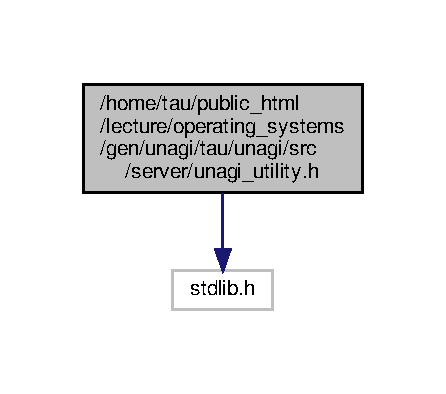
\includegraphics[width=214pt]{unagi__utility_8h__incl}
\end{center}
\end{figure}
This graph shows which files directly or indirectly include this file\+:\nopagebreak
\begin{figure}[H]
\begin{center}
\leavevmode
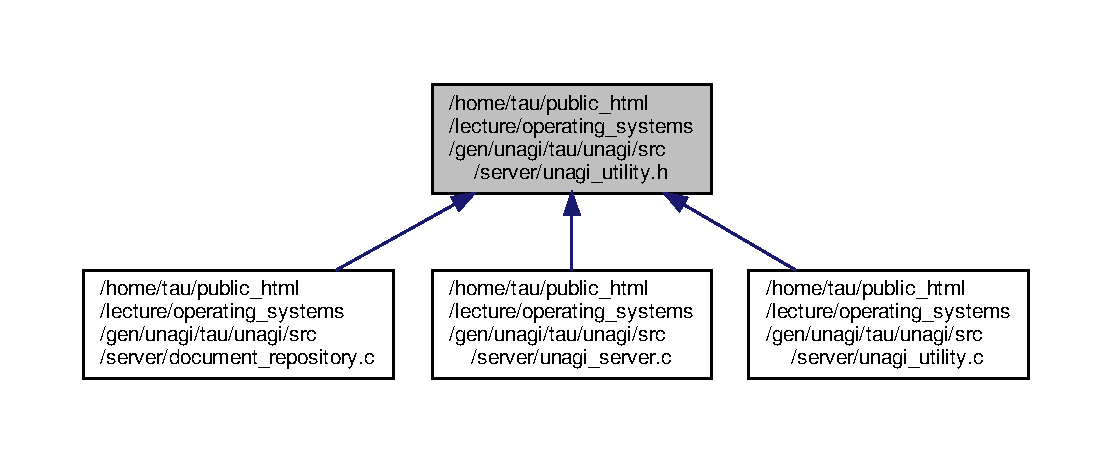
\includegraphics[width=350pt]{unagi__utility_8h__dep__incl}
\end{center}
\end{figure}
\subsection*{Macros}
\begin{DoxyCompactItemize}
\item 
\#define \hyperlink{unagi__utility_8h_a05e8db6b57ab3498eb370a958c2ec6cc}{api\+\_\+err}(msg)~\hyperlink{unagi__utility_8h_a6f52d6a6178c8fbb9e4393d00911c6b5}{api\+\_\+err\+\_\+}(msg, \+\_\+\+\_\+\+F\+I\+L\+E\+\_\+\+\_\+, \+\_\+\+\_\+\+L\+I\+N\+E\+\_\+\+\_\+)
\begin{DoxyCompactList}\small\item\em システムコールや\+C標準関数のエラーメッセージをファイル番号\+:行番号とともに表示 \end{DoxyCompactList}\item 
\#define \hyperlink{unagi__utility_8h_a549b1d478b90fcd78b3aa4d9e9fd9b4f}{internal\+\_\+err}(msg)~\hyperlink{unagi__utility_8h_aa728038408058b42e2a43e01722cbd49}{internal\+\_\+err\+\_\+}(msg, \+\_\+\+\_\+\+F\+I\+L\+E\+\_\+\+\_\+, \+\_\+\+\_\+\+L\+I\+N\+E\+\_\+\+\_\+)
\begin{DoxyCompactList}\small\item\em 内部的なエラーを表示 \end{DoxyCompactList}\end{DoxyCompactItemize}
\subsection*{Functions}
\begin{DoxyCompactItemize}
\item 
void \hyperlink{unagi__utility_8h_a6f52d6a6178c8fbb9e4393d00911c6b5}{api\+\_\+err\+\_\+} (const char $\ast$msg, const char $\ast$\+\_\+\+\_\+file\+\_\+\+\_\+, int \+\_\+\+\_\+line\+\_\+\+\_\+)
\begin{DoxyCompactList}\small\item\em マクロ api\+\_\+err を参照 \end{DoxyCompactList}\item 
void \hyperlink{unagi__utility_8h_aa728038408058b42e2a43e01722cbd49}{internal\+\_\+err\+\_\+} (const char $\ast$msg, const char $\ast$\+\_\+\+\_\+file\+\_\+\+\_\+, int \+\_\+\+\_\+line\+\_\+\+\_\+)
\begin{DoxyCompactList}\small\item\em マクロ internal\+\_\+err を参照 \end{DoxyCompactList}\item 
void $\ast$ \hyperlink{unagi__utility_8h_a7f6cb815cae2536139cd0315633f713b}{malloc\+\_\+or\+\_\+err} (size\+\_\+t sz)
\begin{DoxyCompactList}\small\item\em mallocし, 失敗したらエラーを表示 \end{DoxyCompactList}\item 
\mbox{\Hypertarget{unagi__utility_8h_ad7a4504082a1eeca5b70e47273d3af6b}\label{unagi__utility_8h_ad7a4504082a1eeca5b70e47273d3af6b}} 
void \hyperlink{unagi__utility_8h_ad7a4504082a1eeca5b70e47273d3af6b}{my\+\_\+free} (void $\ast$a)
\begin{DoxyCompactList}\small\item\em freeの代わりにこれを呼ぶ \end{DoxyCompactList}\end{DoxyCompactItemize}


\subsection{Detailed Description}
共通に使うユーティリティ(ヘッダファイル) 

\begin{DoxyAuthor}{Author}
田浦 
\end{DoxyAuthor}
\begin{DoxyDate}{Date}
Oct. 8, 2018 
\end{DoxyDate}


\subsection{Macro Definition Documentation}
\mbox{\Hypertarget{unagi__utility_8h_a05e8db6b57ab3498eb370a958c2ec6cc}\label{unagi__utility_8h_a05e8db6b57ab3498eb370a958c2ec6cc}} 
\index{unagi\+\_\+utility.\+h@{unagi\+\_\+utility.\+h}!api\+\_\+err@{api\+\_\+err}}
\index{api\+\_\+err@{api\+\_\+err}!unagi\+\_\+utility.\+h@{unagi\+\_\+utility.\+h}}
\subsubsection{\texorpdfstring{api\+\_\+err}{api\_err}}
{\footnotesize\ttfamily \#define api\+\_\+err(\begin{DoxyParamCaption}\item[{}]{msg }\end{DoxyParamCaption})~\hyperlink{unagi__utility_8h_a6f52d6a6178c8fbb9e4393d00911c6b5}{api\+\_\+err\+\_\+}(msg, \+\_\+\+\_\+\+F\+I\+L\+E\+\_\+\+\_\+, \+\_\+\+\_\+\+L\+I\+N\+E\+\_\+\+\_\+)}



システムコールや\+C標準関数のエラーメッセージをファイル番号\+:行番号とともに表示 


\begin{DoxyParams}{Parameters}
{\em (msg)} & 表示したいメッセージ \\
\hline
\end{DoxyParams}
\begin{DoxySeeAlso}{See also}
\hyperlink{unagi__utility_8h_a6f52d6a6178c8fbb9e4393d00911c6b5}{api\+\_\+err\+\_\+}
\end{DoxySeeAlso}
システムコール(send, recv, ...)や\+Cの標準関数(malloc, ...)がエラーになった際, 直後にこの関数を呼ぶと原因が表示される. 使用例\+:

char $\ast$ p = malloc(...);

if(!p) api\+\_\+err(\char`\"{}malloc\char`\"{}); \mbox{\Hypertarget{unagi__utility_8h_a549b1d478b90fcd78b3aa4d9e9fd9b4f}\label{unagi__utility_8h_a549b1d478b90fcd78b3aa4d9e9fd9b4f}} 
\index{unagi\+\_\+utility.\+h@{unagi\+\_\+utility.\+h}!internal\+\_\+err@{internal\+\_\+err}}
\index{internal\+\_\+err@{internal\+\_\+err}!unagi\+\_\+utility.\+h@{unagi\+\_\+utility.\+h}}
\subsubsection{\texorpdfstring{internal\+\_\+err}{internal\_err}}
{\footnotesize\ttfamily \#define internal\+\_\+err(\begin{DoxyParamCaption}\item[{}]{msg }\end{DoxyParamCaption})~\hyperlink{unagi__utility_8h_aa728038408058b42e2a43e01722cbd49}{internal\+\_\+err\+\_\+}(msg, \+\_\+\+\_\+\+F\+I\+L\+E\+\_\+\+\_\+, \+\_\+\+\_\+\+L\+I\+N\+E\+\_\+\+\_\+)}



内部的なエラーを表示 


\begin{DoxyParams}{Parameters}
{\em (msg)} & メッセージ \\
\hline
\end{DoxyParams}
\begin{DoxySeeAlso}{See also}
\hyperlink{unagi__utility_8h_aa728038408058b42e2a43e01722cbd49}{internal\+\_\+err\+\_\+}
\end{DoxySeeAlso}
内部的なエラーが発生した際にエラーメッセージ, ファイル名, 行番号を表示し, 終了する 

\subsection{Function Documentation}
\mbox{\Hypertarget{unagi__utility_8h_a6f52d6a6178c8fbb9e4393d00911c6b5}\label{unagi__utility_8h_a6f52d6a6178c8fbb9e4393d00911c6b5}} 
\index{unagi\+\_\+utility.\+h@{unagi\+\_\+utility.\+h}!api\+\_\+err\+\_\+@{api\+\_\+err\+\_\+}}
\index{api\+\_\+err\+\_\+@{api\+\_\+err\+\_\+}!unagi\+\_\+utility.\+h@{unagi\+\_\+utility.\+h}}
\subsubsection{\texorpdfstring{api\+\_\+err\+\_\+()}{api\_err\_()}}
{\footnotesize\ttfamily void api\+\_\+err\+\_\+ (\begin{DoxyParamCaption}\item[{const char $\ast$}]{msg,  }\item[{const char $\ast$}]{\+\_\+\+\_\+file\+\_\+\+\_\+,  }\item[{int}]{\+\_\+\+\_\+line\+\_\+\+\_\+ }\end{DoxyParamCaption})}



マクロ api\+\_\+err を参照 

\begin{DoxySeeAlso}{See also}
\hyperlink{unagi__utility_8h_a05e8db6b57ab3498eb370a958c2ec6cc}{api\+\_\+err}
\end{DoxySeeAlso}
この関数を直接呼ぶことはない. マクロ api\+\_\+err を参照 
\begin{DoxyParams}{Parameters}
{\em msg} & 表示したいメッセージ \\
\hline
{\em \+\_\+\+\_\+file\+\_\+\+\_\+} & ファイル名 \\
\hline
{\em \+\_\+\+\_\+line\+\_\+\+\_\+} & 行番号 \\
\hline
\end{DoxyParams}
\mbox{\Hypertarget{unagi__utility_8h_aa728038408058b42e2a43e01722cbd49}\label{unagi__utility_8h_aa728038408058b42e2a43e01722cbd49}} 
\index{unagi\+\_\+utility.\+h@{unagi\+\_\+utility.\+h}!internal\+\_\+err\+\_\+@{internal\+\_\+err\+\_\+}}
\index{internal\+\_\+err\+\_\+@{internal\+\_\+err\+\_\+}!unagi\+\_\+utility.\+h@{unagi\+\_\+utility.\+h}}
\subsubsection{\texorpdfstring{internal\+\_\+err\+\_\+()}{internal\_err\_()}}
{\footnotesize\ttfamily void internal\+\_\+err\+\_\+ (\begin{DoxyParamCaption}\item[{const char $\ast$}]{msg,  }\item[{const char $\ast$}]{\+\_\+\+\_\+file\+\_\+\+\_\+,  }\item[{int}]{\+\_\+\+\_\+line\+\_\+\+\_\+ }\end{DoxyParamCaption})}



マクロ internal\+\_\+err を参照 

\begin{DoxySeeAlso}{See also}
\hyperlink{unagi__utility_8h_a549b1d478b90fcd78b3aa4d9e9fd9b4f}{internal\+\_\+err}
\end{DoxySeeAlso}
この関数を直接呼ぶことはない. マクロ internal\+\_\+err を参照 
\begin{DoxyParams}{Parameters}
{\em msg} & 表示したいメッセージ \\
\hline
{\em \+\_\+\+\_\+file\+\_\+\+\_\+} & ファイル名 \\
\hline
{\em \+\_\+\+\_\+line\+\_\+\+\_\+} & 行番号 \\
\hline
\end{DoxyParams}
\mbox{\Hypertarget{unagi__utility_8h_a7f6cb815cae2536139cd0315633f713b}\label{unagi__utility_8h_a7f6cb815cae2536139cd0315633f713b}} 
\index{unagi\+\_\+utility.\+h@{unagi\+\_\+utility.\+h}!malloc\+\_\+or\+\_\+err@{malloc\+\_\+or\+\_\+err}}
\index{malloc\+\_\+or\+\_\+err@{malloc\+\_\+or\+\_\+err}!unagi\+\_\+utility.\+h@{unagi\+\_\+utility.\+h}}
\subsubsection{\texorpdfstring{malloc\+\_\+or\+\_\+err()}{malloc\_or\_err()}}
{\footnotesize\ttfamily void$\ast$ malloc\+\_\+or\+\_\+err (\begin{DoxyParamCaption}\item[{size\+\_\+t}]{sz }\end{DoxyParamCaption})}



mallocし, 失敗したらエラーを表示 

szバイトをmallocで割り当てる. 失敗したらエラーを表示(して\+N\+U\+L\+Lを返す. 終了はしない) 
\begin{DoxyParams}{Parameters}
{\em sz} & 割当量(バイト数) \\
\hline
\end{DoxyParams}

%--- End generated contents ---

% Index
\backmatter
\newpage
\phantomsection
\clearemptydoublepage
\addcontentsline{toc}{chapter}{Index}
\printindex

\end{document}
